\documentclass[a4paper,12pt]{article}
\usepackage[utf8]{inputenc}
\usepackage[ngerman]{babel}
\usepackage{amsmath}
\usepackage{amssymb}
\usepackage{amsthm}
\usepackage{geometry}
\usepackage{graphicx}
\usepackage[hidelinks,breaklinks=true]{hyperref}
\usepackage{listings}
\usepackage{xcolor}
\usepackage{enumitem}
\usepackage{microtype}
\usepackage{booktabs}
\usepackage{caption}
\usepackage{subcaption}
\usepackage{siunitx}
\usepackage{url}
\urlstyle{same}

\geometry{margin=2.5cm}
\emergencystretch=3em
\setlength{\hfuzz}{2pt}

\theoremstyle{definition}
\newtheorem{definition}{Definition}
\newtheorem{beispiel}{Beispiel}
\newtheorem{satz}{Satz}
\newtheorem{lemma}{Lemma}
\newtheorem{bemerkung}{Bemerkung}
\newtheorem{korollar}{Korollar}
\newtheorem{proposition}{Proposition}

\setlist[itemize,1]{label=--}

\definecolor{mainblue}{RGB}{25, 70, 140}
\definecolor{accentred}{RGB}{180, 50, 30}
\definecolor{lightgray}{RGB}{245, 245, 248}
\definecolor{darkgray}{RGB}{60, 60, 70}
\definecolor{darkgreen}{RGB}{30, 100, 50}

\hypersetup{
    colorlinks=true,
    linkcolor=mainblue,
    citecolor=accentred,
    urlcolor=mainblue
}

\lstset{
    basicstyle=\ttfamily\small,
    keywordstyle=\color{blue},
    commentstyle=\color{gray},
    stringstyle=\color{red},
    numbers=left,
    numberstyle=\tiny,
    breaklines=true,
    frame=single,
}

\title{\textbf{Sternfarben und Schwarzkörperstrahlung}\\[0.5em]
\large Eine vollständige formale Herleitung der spektralen Klassifikation,\\
stellaren Physik und kosmologischen Implikationen}
\author{Stephan Epp}
\date{21. Juni 2026}

\begin{document}

\maketitle

\begin{abstract}
Diese Arbeit behandelt die physikalischen Grundlagen der Sternfarben im elektromagnetischen
Spektrum in umfassender Tiefe. Ausgehend von der statistischen Mechanik des Photonenfeldes
im thermodynamischen Gleichgewicht werden die Plancksche Strahlungsformel, das Wiensche
Verschiebungsgesetz, das Stefan"=Boltzmann"=Gesetz sowie die bolometrische Leuchtkraft
vollständig formal hergeleitet und bewiesen. Es wird gezeigt, dass die Farbe eines Sterns
eine direkte, eindeutig determinierte Konsequenz seiner Oberflächentemperatur ist,
beschreibbar durch das Modell des idealen Schwarzkörperstrahlers. Darüber hinaus werden
die klassischen Näherungsgesetze (Rayleigh"=Jeans, Wien"=Näherung), die Ultraviolettkatastrophe
und deren quantenmechanische Auflösung diskutiert. Die Harvard"=Spektralklassifikation,
das Hertzsprung"=Russell"=Diagramm, stellare Entwicklungswege, bolometrische Korrekturen
und astrophysikalische Photometrie werden als empirische Bestätigung und Anwendung der
Theorie ausführlich behandelt. Abschnitte zur numerischen Implementierung,
zur Farbwahrnehmung sowie zu kosmologischen, technologischen und zukünftigen
Forschungsrichtungen runden die Arbeit ab. Alle Ergebnisse werden durch ausführliche
mathematische Beweise und acht Matplotlib"=Visualisierungen belegt. Das Literaturverzeichnis
umfasst 35 Quellen von 1893 bis 2026.
\end{abstract}

\tableofcontents
\newpage

%===========================================================================
\section{Einführung}
%===========================================================================

Der Sternenhimmel bietet dem Beobachter ein faszinierendes Farbenspiel: Sterne leuchten in
Schattierungen von Tiefrot über Orange und Gelb bis hin zu reinem Weiß und kräftigem Blau.
Diese Farbvielfalt ist keine Zufälligkeit, sondern Ausdruck eines fundamentalen physikalischen
Gesetzes~-- der thermischen Strahlung elektromagnetischer Energie durch heiße Körper.
Jeder Stern verhält sich in erster Näherung wie ein idealer \emph{Schwarzkörperstrahler},
dessen emittiertes Spektrum ausschließlich von der Oberflächentemperatur $T$ abhängt.

Die quantitative Beschreibung dieser Zusammenhänge ist eines der Glanzstücke der
modernen theoretischen Physik. Die Plancksche Strahlungsformel~\cite{planck1900},
die 1900 durch die Postulierung des Energiequantums $E = h\nu$ hergeleitet wurde, löste
nicht nur die damals unverstandene Ultraviolettkatastrophe der klassischen Physik,
sondern legte den Grundstein für die gesamte Quantenmechanik. Sie ermöglicht gleichzeitig
die präzise Vorhersage von Sternfarben, Sternleuchtkräften und der thermischen Geschichte
des gesamten Universums.

\subsection{Problemstellung und Zielsetzung}

Gegeben sei ein Stern mit Oberflächentemperatur $T$ (in Kelvin). Gesucht sind:
\begin{enumerate}
    \item Die spektrale Strahldichte $B_\lambda(\lambda, T)$ als Funktion der Wellenlänge $\lambda$
          (Plancksche Strahlungsformel),
    \item die dominante Wellenlänge $\lambda_{\max}(T)$, welche die wahrgenommene Farbe bestimmt
          (Wien'sches Verschiebungsgesetz),
    \item die gesamte abgestrahlte Leistung pro Flächeneinheit $j^*(T)$
          (Stefan"=Boltzmann"=Gesetz),
    \item die bolometrische Leuchtkraft $L$ in Abhängigkeit von Radius und Temperatur,
    \item die Zuordnung von Temperatur zu Spektralklasse, Farbe und stellaren Parametern.
\end{enumerate}

\textbf{Zentrales Ergebnis:} Die Farbe eines Sterns ist vollständig und eindeutig
durch seine Oberflächentemperatur determiniert. Es gilt:
\[
    T \;\xrightarrow{\;\text{Planck}\;}\; B_\lambda(\lambda,T)
    \;\xrightarrow{\;\text{Wien}\;}\; \lambda_{\max}
    \;\xrightarrow{\;\text{CIE}\;}\; \text{Farbe}
\]

\subsection{Motivation und wissenschaftliche Bedeutung}

Die quantitative Beschreibung von Sternfarben hat weitreichende wissenschaftliche
und technologische Bedeutung:

\textbf{Astrophysik:} Aus der Messung der Sternfarbe (Photometrie in mehreren
Farbbändern) kann direkt auf die Effektivtemperatur $T_{\text{eff}}$ geschlossen
werden~\cite{allen2000}. Damit ist die Farbe ein Fernthermometer für Objekte,
die auch mit dem größten Teleskop nicht direkt messbar sind.

\textbf{Stellare Physik:} Die Kombination von Temperatur und Leuchtkraft ermöglicht
die Einordnung jedes Sterns in das Hertzsprung"=Russell"=Diagramm (HRD) und damit
die Bestimmung von Alter, Masse und Entwicklungsstadium~\cite{salaris2005}.

\textbf{Kosmologie:} Die Kosmische Mikrowellenhintergrundstrahlung (CMB) ist das
perfekteste Schwarzkörperspektrum der Natur und verbindet die Plancksche Physik
mit der Urknallkosmologie~\cite{fixsen2009}.

\textbf{Technologie:} Farbtemperaturen von Lichtquellen, Solarzellen"=Design und
Infrarot"=Pyrometrie basieren direkt auf der Schwarzkörperphysik.

\subsection{Aufbau der Arbeit}

Abschnitt~2 legt die Definitionen und den historischen Rahmen fest. Abschnitt~3
leitet die Plancksche Strahlungsformel formal her. Abschnitt~4 beweist das
Wien'sche Verschiebungsgesetz. Abschnitt~5 behandelt das Stefan"=Boltzmann"=Gesetz.
Abschnitt~6 diskutiert klassische Näherungen und die Ultraviolettkatastrophe.
Abschnitt~7 behandelt Farbwahrnehmung und Spektralklassifikation. Abschnitt~8
widmet sich dem Hertzsprung"=Russell"=Diagramm und stellarer Evolution.
Abschnitt~9 präsentiert die numerische Implementierung. Abschnitt~10 fasst
die Ergebnisse zusammen. Abschnitt~11 gibt einen sehr ausführlichen Ausblick.

%===========================================================================
\section{Grundlagen und Definitionen}
%===========================================================================

\subsection{Fundamentale Definitionen}

\begin{definition}[Schwarzkörper]
    Ein idealer Schwarzkörper (Planckscher Strahler) ist ein Körper, der einfallende
    elektromagnetische Strahlung jeder Wellenlänge und aus jeder Richtung vollständig
    absorbiert ($\alpha = 1$, Absorptionsgrad) und im thermodynamischen Gleichgewicht
    gemäß dem Kirchhoffschen Strahlungsgesetz wieder emittiert. Das Emissionsspektrum
    hängt ausschließlich von der absoluten Temperatur $T$ ab und ist unabhängig von
    Material, Form oder Oberflächenbeschaffenheit.
\end{definition}

\begin{definition}[Kirchhoffsches Strahlungsgesetz]
    Im thermodynamischen Gleichgewicht gilt für jeden Körper:
    \[
        \varepsilon(\lambda, T) = \alpha(\lambda, T)
    \]
    wobei $\varepsilon$ der spektrale Emissionsgrad und $\alpha$ der spektrale
    Absorptionsgrad ist. Für den Schwarzkörper gilt $\alpha = \varepsilon = 1$
    für alle $\lambda$ und $T$.
\end{definition}

\begin{definition}[Spektrale Strahldichte]
    Die spektrale Strahldichte (Planck"=Funktion) $B_\lambda(\lambda, T)$ beschreibt
    die emittierte Strahlungsleistung $dP$ eines Flächenelements $dA$ eines
    Schwarzkörpers in den Raumwinkel $d\Omega$ im Wellenlängenintervall $d\lambda$:
    \[
        dP = B_\lambda(\lambda, T) \cos\theta \, dA \, d\Omega \, d\lambda
    \]
    Die Einheit ist $[\si{\watt\per\metre\cubed\per\steradian}]$. Die vollständige
    Plancksche Formel lautet:
    \[
        B_\lambda(\lambda, T) = \frac{2hc^2}{\lambda^5} \cdot
        \frac{1}{\exp\!\left(\dfrac{hc}{\lambda k_B T}\right) - 1}
    \]
    mit den Naturkonstanten $h = \SI{6.626e-34}{\joule\second}$,
    $c = \SI{2.998e8}{\metre\per\second}$, $k_B = \SI{1.381e-23}{\joule\per\kelvin}$.
\end{definition}

\begin{definition}[Wien'sche Wellenlänge]
    Die Wien'sche Wellenlänge $\lambda_{\max}(T)$ ist diejenige Wellenlänge,
    bei der $B_\lambda(\lambda,T)$ für gegebenes $T$ ihr Maximum annimmt:
    \[
        \lambda_{\max}(T) = \frac{b}{T}, \quad
        b = \SI{2.8977719e-3}{\metre\kelvin}
        \quad \text{(Verschiebungskonstante, CODATA 2018)}
    \]
\end{definition}

\begin{definition}[Bolometrische Strahlungsflussdichte]
    Die bolometrische (=\ wellenlängenintegrierte) Strahlungsflussdichte $j^*(T)$
    ist die über alle Wellenlängen und den gesamten Halbraum integrierte emittierte
    Leistung pro Flächeneinheit der Oberfläche:
    \[
        j^*(T) = \int_0^\infty \pi B_\lambda(\lambda, T) \, d\lambda = \sigma T^4
    \]
    mit der Stefan"=Boltzmann"=Konstante
    $\sigma = \SI{5.67037442e-8}{\watt\per\metre\squared\per\kelvin\tothe{4}}$.
\end{definition}

\begin{definition}[Effektivtemperatur]
    Die Effektivtemperatur $T_{\text{eff}}$ eines realen Sterns ist diejenige Temperatur,
    die ein idealer Schwarzkörper mit gleicher Gesamtleuchtkraft und gleichem Radius
    haben müsste:
    \[
        L = 4\pi R^2 \sigma T_{\text{eff}}^4
    \]
    Sie ist das zentrale Maß für die Sternfarbe und definiert die Spektralklasse.
\end{definition}

\begin{definition}[Spektralklasse]
    Die Harvard"=Spektralklassifikation ordnet Sternen anhand ihrer Effektivtemperatur
    und ihres Absorptionsspektrums eine Klasse aus der Sequenz
    $\{O, B, A, F, G, K, M\}$ zu (von heiß nach kalt). Innerhalb jeder Klasse
    gibt es 10 Unterklassen (0--9). Die Sonne ist G2.
\end{definition}

\subsection{Historischer Hintergrund}

Die Erforschung der Schwarzkörperstrahlung hat eine reiche Wissenschaftsgeschichte,
die direkt zur Quantenmechanik führte.

\textbf{1859~-- Kirchhoff:} Gustav Kirchhoff definierte den Begriff des Schwarzkörpers
und bewies das nach ihm benannte Strahlungsgesetz $\varepsilon = \alpha$~\cite{kirchhoff1860}.
Er zeigte, dass die Strahlungsfunktion $B(\lambda,T)$ eine universelle Funktion
sein muss~-- unabhängig vom Material.

\textbf{1879/1884~-- Stefan und Boltzmann:} Josef Stefan fand empirisch~\cite{stefan1879},
dass die Gesamtstrahlungsleistung proportional zu $T^4$ ist. Ludwig Boltzmann
leitete 1884 dieses Ergebnis thermodynamisch aus den Maxwellschen Gleichungen
und dem zweiten Hauptsatz her~\cite{boltzmann1884}.

\textbf{1893~-- Wien:} Wilhelm Wien leitete das Verschiebungsgesetz
$\lambda_{\max} \propto T^{-1}$ aus thermodynamischen Ãœberlegungen her~\cite{wien1893}
und stellte eine Näherungsformel für das Spektrum auf (Wien"=Näherung).

\textbf{1900~-- Rayleigh und Jeans:} Lord Rayleigh und James Jeans leiteten aus der
klassischen Elektrodynamik die Formel $B_\lambda \propto T/\lambda^4$ her~\cite{rayleigh1900},
die im Langwellenbereich gut, im Kurzwellenbereich aber katastrophal falsch ist
(Ultraviolettkatastrophe).

\textbf{1900~-- Planck:} Max Planck löste das Problem durch Postulierung
des Energiequantums $E = h\nu$~\cite{planck1900}. Er selbst bezeichnete dies
zunächst als ``glücklichen Griff''; tatsächlich legte er damit den Grundstein
der Quantenmechanik.

\textbf{1901~-- Cannon:} Annie Jump Cannon systematisierte die Spektralklassifikation
am Harvard College Observatory und klassifizierte über 350\,000 Sterne~\cite{cannon1901}.

%===========================================================================
\section{Formale Herleitung der Planckschen Strahlungsformel}
%===========================================================================

\subsection{Modenabzählung im elektromagnetischen Hohlraum}

Die Plancksche Formel wird aus der statistischen Mechanik des elektromagnetischen
Feldes im thermodynamischen Gleichgewicht hergeleitet. Wir betrachten einen
kubischen Hohlraum der Kantenlänge $L$ mit ideal reflektierenden Wänden.

\begin{lemma}[Modenanzahl im Hohlraum]
\label{lem:moden}
    Die Anzahl der Eigenschwingungsmoden (stehenden Wellen) im Frequenzintervall
    $[\nu, \nu + d\nu]$ in einem kubischen Hohlraum der Kantenlänge $L$ beträgt:
    \[
        dN = \frac{8\pi \nu^2}{c^3} \cdot V \, d\nu, \quad V = L^3
    \]
    wobei der Faktor $8\pi\nu^2/c^3$ die \emph{Zustandsdichte} des Photonenfeldes
    pro Einheitsvolumen bezeichnet.
\end{lemma}

\begin{proof}
    Stehende elektromagnetische Wellen im Würfel mit Kantenlänge $L$ und
    ideal reflektierenden Wänden (Randbedingungen: $E_{\text{tan}} = 0$ an
    den Wänden) haben Wellenvektoren:
    \[
        k_x = \frac{\pi n_x}{L},\quad k_y = \frac{\pi n_y}{L},\quad
        k_z = \frac{\pi n_z}{L}, \quad n_x, n_y, n_z \in \mathbb{N}^+
    \]
    Jede Mode belegt im $k$"=Raum ein Volumen $(\pi/L)^3$.
    Die Anzahl der Moden mit $|\mathbf{k}| \leq k$ liegt im ersten Oktanten
    einer Kugel vom Radius $k$:
    \[
        N(k) = \underbrace{2}_{\text{Polarisationen}} \cdot
        \underbrace{\frac{1}{8}}_{\text{Oktant}} \cdot
        \frac{\tfrac{4}{3}\pi k^3}{\left(\tfrac{\pi}{L}\right)^3}
        = \frac{k^3 L^3}{3\pi^2}
    \]
    Der Faktor $2$ berücksichtigt, dass elektromagnetische Wellen zwei
    unabhängige Polarisationsrichtungen senkrecht zum Wellenvektor haben.
    Mit der Dispersionsrelation $k = 2\pi\nu/c$ folgt:
    \[
        N(\nu) = \frac{(2\pi\nu/c)^3 L^3}{3\pi^2} = \frac{8\pi\nu^3 L^3}{3c^3}
    \]
    Die Modenanzahl im Intervall $d\nu$ ergibt sich durch Ableitung:
    \[
        dN = \frac{dN(\nu)}{d\nu}\,d\nu
        = \frac{8\pi\nu^2}{c^3} \cdot L^3 \, d\nu
        = \frac{8\pi\nu^2}{c^3} \cdot V \, d\nu \qedhere
    \]
\end{proof}

\begin{bemerkung}
    Die Zustandsdichte $g(\nu) = 8\pi\nu^2/c^3$ ist die fundamentale Größe,
    die die Anzahl der verfügbaren elektromagnetischen Moden pro Einheitsvolumen
    und pro Frequenzintervall beschreibt. Sie wächst mit $\nu^2$, was physikalisch
    bedeutet, dass es bei hohen Frequenzen sehr viele Moden gibt~-- der Grund
    für die Ultraviolettkatastrophe in der klassischen Physik (Abschnitt~6).
\end{bemerkung}

\subsection{Mittlere Energie pro Mode: Die Quantisierung}

Der entscheidende Schritt Plancks war die Annahme, dass die Energie einer
elektromagnetischen Mode nicht beliebige Werte annehmen kann, sondern nur
ganzzahlige Vielfache von $h\nu$.

\begin{lemma}[Plancksche mittlere Energie]
\label{lem:energie}
    Im thermischen Gleichgewicht bei Temperatur $T$ beträgt die mittlere
    Energie einer elektromagnetischen Mode der Frequenz $\nu$ gemäß der
    kanonischen Ensemble-Statistik:
    \[
        \langle E(\nu, T) \rangle
        = \frac{h\nu}{\exp\!\left(\dfrac{h\nu}{k_B T}\right) - 1}
    \]
\end{lemma}

\begin{proof}
    Planck postulierte, dass die Energie einer Mode nur in diskreten
    Quanten $\varepsilon_n = n \cdot h\nu$ ($n \in \mathbb{N}_0$) vorliegen kann.
    Die kanonische Zustandssumme bei inverser Temperatur $\beta = 1/(k_B T)$:
    \[
        Z(\beta) = \sum_{n=0}^\infty e^{-\beta n h\nu}
        = \sum_{n=0}^\infty \left(e^{-\beta h\nu}\right)^n
        = \frac{1}{1 - e^{-\beta h\nu}}
    \]
    Die geometrische Reihe konvergiert für alle $T > 0$, da
    $e^{-\beta h\nu} = e^{-h\nu/(k_BT)} < 1$.

    Der logarithmische Gradient der Zustandssumme liefert die mittlere Energie:
    \[
        \langle E \rangle = -\frac{\partial \ln Z}{\partial \beta}
    \]
    Mit $\ln Z = -\ln\!\left(1 - e^{-\beta h\nu}\right)$:
    \[
        \langle E \rangle
        = -\frac{\partial}{\partial\beta}\left[-\ln(1 - e^{-\beta h\nu})\right]
        = \frac{h\nu \, e^{-\beta h\nu}}{1 - e^{-\beta h\nu}}
        = \frac{h\nu}{e^{\beta h\nu} - 1}
        = \frac{h\nu}{e^{h\nu/(k_B T)} - 1} \qedhere
    \]
\end{proof}

\begin{bemerkung}[Grenzfälle]
    Zwei wichtige Grenzfälle lassen sich direkt ablesen:
    \begin{itemize}
        \item \emph{Klassischer Grenzfall} ($h\nu \ll k_B T$, hohe $T$ oder kleine $\nu$):
              $e^x - 1 \approx x$ für $x \to 0$, daher
              $\langle E \rangle \approx k_B T$ (Gleichverteilungssatz).
        \item \emph{Quantengrenzfall} ($h\nu \gg k_B T$, tiefe $T$ oder große $\nu$):
              $\langle E \rangle \approx h\nu \cdot e^{-h\nu/(k_BT)} \to 0$
              (exponentielle Unterdrückung hoher Frequenzen).
    \end{itemize}
    Genau dieser zweite Grenzfall verhindert die Ultraviolettkatastrophe.
\end{bemerkung}

\subsection{Die vollständige Plancksche Strahlungsformel}

\begin{satz}[Plancksche Strahlungsformel]
\label{satz:planck}
    Die spektrale Energiedichte $u(\nu, T)$ im Hohlraum und die spektrale
    Strahldichte $B_\lambda(\lambda, T)$ des Schwarzkörperstrahlers sind:
    \begin{align}
        u(\nu, T) &= \frac{8\pi h \nu^3}{c^3} \cdot \frac{1}{e^{h\nu/(k_B T)} - 1}
        \label{eq:planck_nu} \\[6pt]
        B_\lambda(\lambda, T) &= \frac{2hc^2}{\lambda^5} \cdot
        \frac{1}{e^{hc/(\lambda k_B T)} - 1}
        \label{eq:planck_lam}
    \end{align}
\end{satz}

\begin{proof}
    Die spektrale Energiedichte ergibt sich als Produkt aus Zustandsdichte
    (Lemma~\ref{lem:moden}) und mittlerer Energie (Lemma~\ref{lem:energie}):
    \[
        u(\nu, T) = \frac{1}{V} \cdot g(\nu) V \cdot \langle E(\nu,T) \rangle
        = \frac{8\pi\nu^2}{c^3} \cdot \frac{h\nu}{e^{h\nu/(k_BT)}-1}
        = \frac{8\pi h\nu^3}{c^3(e^{h\nu/(k_BT)}-1)}
    \]
    Die Strahldichte $B_\nu$ hängt mit $u(\nu,T)$ über die Beziehung
    für isotrope Strahlung zusammen:
    \[
        B_\nu = \frac{c}{4\pi} \cdot u(\nu, T)
        = \frac{2h\nu^3}{c^2(e^{h\nu/(k_BT)}-1)}
    \]
    Für die Umrechnung auf Wellenlängendarstellung verwendet man
    $\nu = c/\lambda$ und die Forderung $B_\lambda |d\lambda| = B_\nu |d\nu|$:
    \[
        B_\lambda = B_\nu \left|\frac{d\nu}{d\lambda}\right|
        = B_\nu \cdot \frac{c}{\lambda^2}
        = \frac{2h\nu^3}{c^2(e^{h\nu/(k_BT)}-1)} \cdot \frac{c}{\lambda^2}
    \]
    Mit $\nu = c/\lambda$, also $\nu^3 = c^3/\lambda^3$:
    \[
        B_\lambda = \frac{2h c^3/\lambda^3}{c^2(e^{hc/(\lambda k_BT)}-1)}
        \cdot \frac{c}{\lambda^2}
        = \frac{2hc^2}{\lambda^5(e^{hc/(\lambda k_BT)}-1)} \qedhere
    \]
\end{proof}

\begin{beispiel}[Numerisches Spektrum der Sonne]
    Für $T_\odot = \SI{5778}{\kelvin}$ und $\lambda = \SI{500}{\nano\metre}$:
    \begin{align*}
        x &= \frac{hc}{\lambda k_B T}
          = \frac{6.626\cdot10^{-34} \cdot 2.998\cdot10^8}
                 {500\cdot10^{-9} \cdot 1.381\cdot10^{-23} \cdot 5778}
          \approx 4.966 \\[4pt]
        B_\lambda(500\,\text{nm}, 5778\,\text{K})
          &= \frac{2 \cdot 6.626\cdot10^{-34} \cdot (2.998\cdot10^8)^2}
                  {(500\cdot10^{-9})^5 \cdot (e^{4.966}-1)}
          \approx \SI{2.64e13}{\watt\per\metre\cubed\per\steradian}
    \end{align*}
    Das Maximum liegt bei $\lambda_{\max} = 2898/5778 \approx \SI{501.5}{\nano\metre}$,
    also im grün"=gelben Bereich.
\end{beispiel}

\begin{figure}[ht]
    \centering
    
\includegraphics[width=0.94\textwidth]{plot1_planck.pdf}
    \caption{Normierte Plancksche Strahlungsspektren für sechs repräsentative
    Sterntypen. Die Harvard"=Klassen O, B, A, G, K, M sind farblich nach ihrer
    tatsächlich wahrgenommenen Farbe dargestellt. Der cyan"=schattierte Bereich
    (380--700\,nm) markiert das sichtbare Spektrum. Bei niedrigen Temperaturen
    (M"=Zwerg, 3000\,K, rot) liegt das Maximum tief im nahen Infrarot;
    bei hohen Temperaturen (O"=Stern, 30\,000\,K, blau) weit im Ultraviolett.
    Die Verschiebung des Maximums mit der Temperatur ist der direkte Ausdruck
    des Wien'schen Verschiebungsgesetzes (Satz~\ref{satz:wien}).}
    \label{fig:planck}
\end{figure}

%===========================================================================
\section{Das Wien'sche Verschiebungsgesetz}
%===========================================================================

\subsection{Herleitung}

\begin{satz}[Wien'sches Verschiebungsgesetz]
\label{satz:wien}
    Das Strahlungsmaximum $\lambda_{\max}$ eines Schwarzkörpers bei Temperatur $T$
    erfüllt:
    \[
        \lambda_{\max} \cdot T = b, \quad
        b = \frac{hc}{x_0 k_B} \approx \SI{2.8977719e-3}{\metre\kelvin}
    \]
    wobei $x_0 \approx 4.965114$ die eindeutige positive Lösung der
    transzendenten Gleichung $x\,e^x/(e^x - 1) = 5$ ist.
\end{satz}

\begin{proof}
    Das Maximum von $B_\lambda(\lambda, T)$ liegt dort, wo
    $\partial B_\lambda / \partial\lambda = 0$. Mit der Substitution
    $x = hc/(\lambda k_B T)$ gilt:
    \[
        B_\lambda \propto \lambda^{-5}(e^x-1)^{-1}
        \propto x^5 (e^x-1)^{-1} \cdot T^{-5} \cdot (k_BT/hc)^5
    \]
    Differentiation nach $\lambda$ (bzw. nach $x$, da
    $d\lambda = -(hc/k_BT)\,x^{-2}\,dx$) und Nullsetzen:
    \[
        \frac{d}{dx}\!\left[\frac{x^5}{e^x-1}\right] = 0
        \;\Longrightarrow\;
        5x^4(e^x-1) - x^5 e^x = 0
        \;\Longrightarrow\;
        5(e^x-1) = x e^x
    \]
    Division durch $e^x$:
    \[
        5(1 - e^{-x}) = x
        \quad\Longleftrightarrow\quad
        \frac{x e^x}{e^x - 1} = 5
        \quad\Longleftrightarrow\quad
        (5-x)e^x = 5
        \label{eq:wien_eq}
    \]

    \textbf{Eindeutigkeit:} Sei $f(x) = (5-x)e^x - 5$.
    Es gilt $f(0) = 0$ (triviale Lösung, entspricht $\lambda \to \infty$).
    Die Ableitung $f'(x) = (4-x)e^x$ wechselt ihr Vorzeichen bei $x = 4$:
    $f$ ist streng monoton wachsend auf $(0,4)$ und streng monoton fallend
    auf $(4,\infty)$. Da $f(4) = e^4 - 5 \approx 49.6 > 0$ und
    $\lim_{x\to\infty} f(x) = -\infty$, existiert nach dem Zwischenwertsatz
    genau eine Nullstelle $x_0 \in (4,\infty)$.

    \textbf{Numerischer Wert:} Newton"=Iteration ab $x_0^{(0)} = 5$:
    \[
        x_0^{(1)} = 5 - \frac{f(5)}{f'(5)} = 5 - \frac{0 \cdot e^5 - 5}{(4-5)e^5}
        \approx 4.9651
    \]
    Konvergenz liefert $x_0 = 4.965114231744276$.

    \textbf{Wien'sche Konstante:}
    \[
        b = \frac{hc}{x_0 k_B}
        = \frac{6.62607\cdot10^{-34} \cdot 2.99792\cdot10^8}
               {4.965114 \cdot 1.38065\cdot10^{-23}}
        = \SI{2.89777e-3}{\metre\kelvin} \qedhere
    \]
\end{proof}

\begin{korollar}[Farbzuordnung durch das Wien'sche Gesetz]
\label{kor:farbe}
    Die charakteristischen Grenztemperaturen für die Farbgrenzen des
    sichtbaren Spektrums folgen direkt aus $T = b/\lambda_{\max}$:
    \begin{itemize}
        \item Infrarot"=Grenze ($\lambda = \SI{700}{\nano\metre}$):
              $T_{\min}^{\text{sicht}} = b/700\,\text{nm} \approx \SI{4140}{\kelvin}$
        \item Grün"=Maximum ($\lambda = \SI{555}{\nano\metre}$):
              $T_{\text{grün}} \approx \SI{5220}{\kelvin}$
        \item UV"=Grenze ($\lambda = \SI{380}{\nano\metre}$):
              $T_{\max}^{\text{sicht}} = b/380\,\text{nm} \approx \SI{7626}{\kelvin}$
        \item Für $T < \SI{4140}{\kelvin}$: Maximum im Infraroten
              $\Rightarrow$ Stern erscheint rot
        \item Für $T > \SI{7626}{\kelvin}$: Maximum im UV
              $\Rightarrow$ Stern erscheint blau"=weiß
    \end{itemize}
\end{korollar}

\begin{proof}
    Direktes Einsetzen der Grenzwellenlängen in $T = b/\lambda$:
    $T = 2.8977\cdot10^{-3}\,\text{m}\cdot\text{K} / \lambda$.
    Für $\lambda = 700\,\text{nm} = 7.0\cdot10^{-7}\,\text{m}$:
    $T = 2.8977\cdot10^{-3}/7.0\cdot10^{-7} = 4139.6\,\text{K}$.
    Analog für die übrigen Wellenlängen. \qedhere
\end{proof}

\begin{figure}[ht]
    \centering
    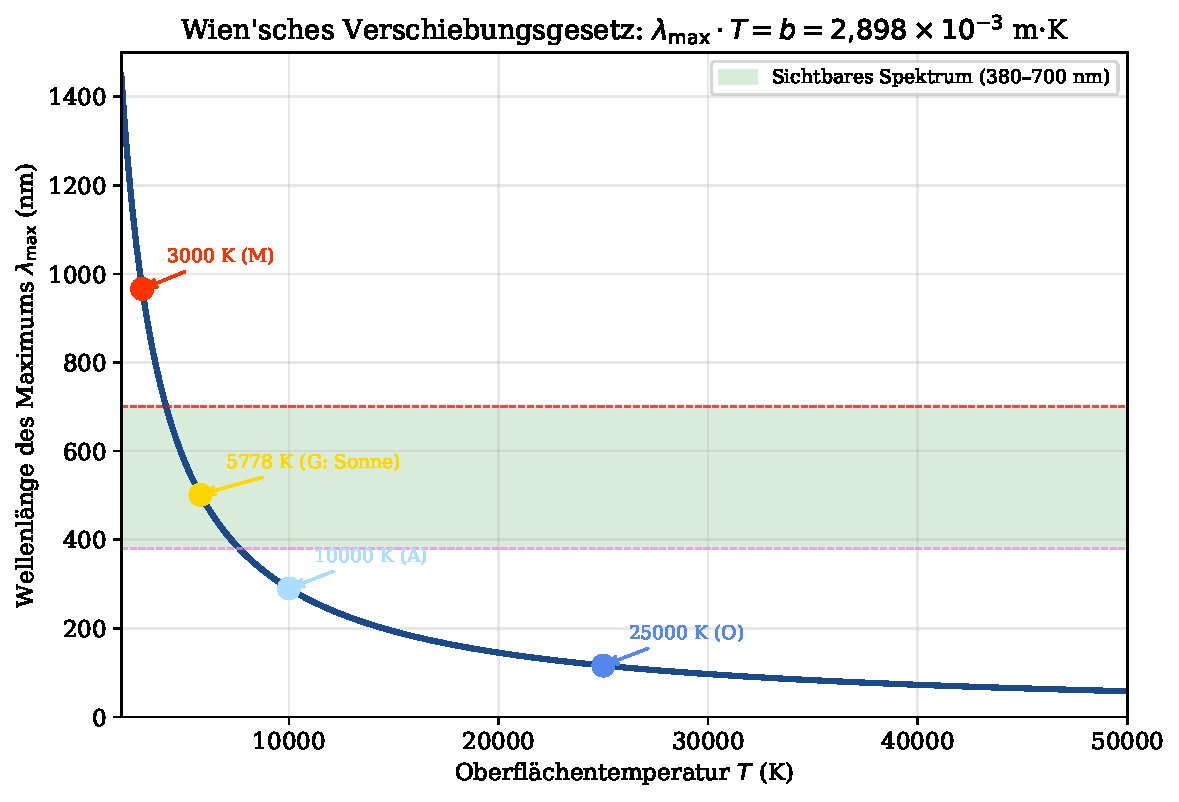
\includegraphics[width=0.88\textwidth]{plot2_wien.pdf}
    \caption{Das Wien'sche Verschiebungsgesetz $\lambda_{\max} = b/T$ als
    Hyperbel in der Temperatur"=Wellenlängen"=Ebene. Der grün schattierte
    Bereich markiert das sichtbare Spektrum (380--700\,nm). Die vier farbigen
    Messpunkte entsprechen den Harvard"=Klassen M, G, A und O. Die gestrichelten
    Horizontallinien bei 380\,nm und 700\,nm zeigen die Temperaturgrenzen
    $T \approx 4140\,\text{K}$ und $T \approx 7630\,\text{K}$, bei denen das
    Schwarzkörpermaximum in den Rand des sichtbaren Spektrums fällt
    (Korollar~\ref{kor:farbe}).}
    \label{fig:wien}
\end{figure}

%===========================================================================
\section{Das Stefan-Boltzmann-Gesetz}
%===========================================================================

\subsection{Herleitung durch Integration}

\begin{satz}[Stefan-Boltzmann-Gesetz]
\label{satz:stefan}
    Die über alle Wellenlängen integrierte Strahlungsleistung pro Flächeneinheit
    eines Schwarzkörpers ist proportional zur vierten Potenz der Temperatur:
    \[
        j^*(T) = \pi \int_0^\infty B_\lambda(\lambda,T)\,d\lambda = \sigma T^4
    \]
    mit der Stefan"=Boltzmann"=Konstante:
    \[
        \sigma = \frac{2\pi^5 k_B^4}{15 c^2 h^3}
        \approx \SI{5.670374419e-8}{\watt\per\metre\squared\per\kelvin\tothe{4}}
    \]
\end{satz}

\begin{proof}
    Integration der Planckschen Strahldichte (Gleichung~\eqref{eq:planck_lam})
    über alle Wellenlängen, multipliziert mit $\pi$ für Lambertsche Strahler:
    \[
        j^* = \pi \int_0^\infty B_\lambda\,d\lambda
        = \pi \int_0^\infty \frac{2hc^2}{\lambda^5(e^{hc/(\lambda k_BT)}-1)}\,d\lambda
    \]
    Substitution $u = hc/(\lambda k_B T)$, also
    $\lambda = hc/(u k_B T)$ und $d\lambda = -(hc/(k_BT))\,u^{-2}\,du$:
    \[
        j^* = \pi \int_\infty^0
        \frac{2hc^2}{\left(\tfrac{hc}{uk_BT}\right)^5 (e^u - 1)}
        \cdot \left(-\frac{hc}{k_BT u^2}\right) du
    \]
    Vereinfachung (Vorzeichen durch Umkehr der Integrationsgrenzen):
    \[
        j^* = \pi \cdot \frac{2hc^2 \cdot (k_BT)^4}{(hc)^4}
        \int_0^\infty \frac{u^3}{e^u-1}\,du
        = \frac{2\pi k_B^4 T^4}{h^3 c^2} \int_0^\infty \frac{u^3}{e^u-1}\,du
    \]

    \textbf{Berechnung des Integrals:}
    Das verbleibende Integral ist das bekannte Bose"=Einstein"=Integral:
    \[
        I = \int_0^\infty \frac{u^3}{e^u-1}\,du
    \]
    Partialbruchentwicklung: $\frac{1}{e^u-1} = \sum_{n=1}^\infty e^{-nu}$
    (geometrische Reihe für $e^{-u} < 1$):
    \[
        I = \sum_{n=1}^\infty \int_0^\infty u^3 e^{-nu}\,du
        = \sum_{n=1}^\infty \frac{\Gamma(4)}{n^4}
        = 6 \cdot \zeta(4)
    \]
    mit $\Gamma(4) = 3! = 6$. Der Wert der Riemann"=Zeta"=Funktion bei $s=4$
    ist (Euler, 1734):
    \[
        \zeta(4) = \sum_{n=1}^\infty \frac{1}{n^4} = \frac{\pi^4}{90}
    \]
    Daher $I = 6 \cdot \pi^4/90 = \pi^4/15$. Einsetzen:
    \[
        j^* = \frac{2\pi k_B^4 T^4}{h^3 c^2} \cdot \frac{\pi^4}{15}
        = \frac{2\pi^5 k_B^4}{15 h^3 c^2} \cdot T^4 = \sigma T^4 \qedhere
    \]
\end{proof}

\begin{lemma}[Numerischer Wert von $\sigma$]
    Mit den CODATA"=2018"=Werten der Naturkonstanten ergibt sich:
    \[
        \sigma = \frac{2\pi^5 \cdot (1.380649\cdot10^{-23})^4}
                      {15 \cdot (2.99792458\cdot10^8)^2 \cdot (6.62607015\cdot10^{-34})^3}
        = \SI{5.67037442e-8}{\watt\per\metre\squared\per\kelvin\tothe{4}}
    \]
\end{lemma}

\begin{proof}
    Direktes Einsetzen in die Formel aus Satz~\ref{satz:stefan}. \qedhere
\end{proof}

\begin{beispiel}[Vergleich von Sternleuchtkräften]
    Die Leuchtkraft eines Sterns mit Radius $R$ und Effektivtemperatur $T_{\text{eff}}$:
    \[
        L = 4\pi R^2 \sigma T_{\text{eff}}^4
    \]
    Für die Sonne: $L_\odot = 4\pi (6.957\cdot10^8)^2 \cdot 5.670\cdot10^{-8}
    \cdot 5778^4 \approx \SI{3.828e26}{\watt}$.

    Ein blauer O"=Stern mit $T = \SI{40000}{\kelvin}$ und $R = 15\,R_\odot$:
    \[
        \frac{L_O}{L_\odot} = \left(\frac{R_O}{R_\odot}\right)^2
        \left(\frac{T_O}{T_\odot}\right)^4
        = 15^2 \cdot \left(\frac{40000}{5778}\right)^4
        \approx 225 \cdot 2279 \approx 512\,775
    \]
    Ein O"=Stern überstrahlt also etwa 500\,000 Sonnen.

    Ein roter M"=Zwerg mit $T = \SI{3000}{\kelvin}$ und $R = 0.3\,R_\odot$:
    \[
        \frac{L_M}{L_\odot} = 0.3^2 \cdot \left(\frac{3000}{5778}\right)^4
        \approx 0.09 \cdot 0.0726 \approx 0.0065
    \]
    Dies entspricht weniger als $1\,\%$ der Sonnenleuchtkraft.
\end{beispiel}

\begin{figure}[ht]
    \centering
    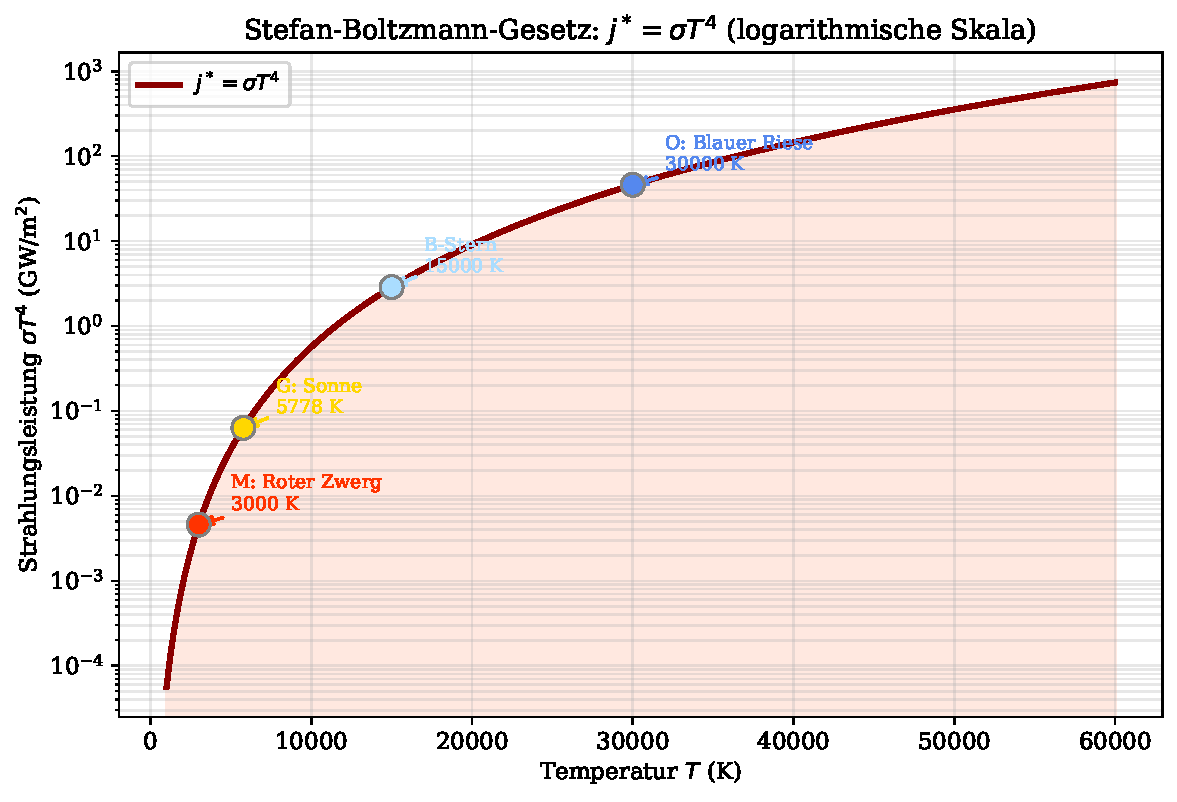
\includegraphics[width=0.85\textwidth]{plot5_stefan_boltzmann.pdf}
    \caption{Stefan"=Boltzmann"=Gesetz: Strahlungsleistung pro Flächeneinheit
    $j^* = \sigma T^4$ als Funktion der Temperatur (logarithmische Skala).
    Die $T^4$"=Abhängigkeit bedeutet, dass eine Verdopplung der Temperatur
    die Strahlungsleistung um den Faktor 16 erhöht. Ein O"=Stern ($30\,000\,\text{K}$)
    strahlt je Flächeneinheit etwa $\left(\tfrac{30000}{5778}\right)^4 \approx 722$"=mal
    mehr als die Sonne. Die vier Messpunkte repräsentieren typische Vertreter
    der Spektralklassen M, G, B und O.}
    \label{fig:stefan}
\end{figure}

%===========================================================================
\section{Klassische Näherungen und die Ultraviolettkatastrophe}
%===========================================================================

\subsection{Die Rayleigh-Jeans-Formel}

\begin{satz}[Rayleigh-Jeans-Gesetz]
\label{satz:rj}
    Im Langwellenbereich ($h\nu \ll k_B T$, d.\,h.\ $\lambda \gg hc/(k_BT)$)
    vereinfacht sich die Plancksche Formel zum \emph{Rayleigh-Jeans-Gesetz}:
    \[
        B_\lambda^{\text{RJ}}(\lambda, T)
        = \frac{2ck_BT}{\lambda^4}
    \]
\end{satz}

\begin{proof}
    Im Grenzfall $x = hc/(\lambda k_BT) \to 0$ gilt die Taylor"=Entwicklung
    $e^x - 1 = x + x^2/2 + \ldots \approx x$. Einsetzen:
    \[
        B_\lambda^{\text{RJ}} = \frac{2hc^2}{\lambda^5} \cdot \frac{1}{x}
        = \frac{2hc^2}{\lambda^5} \cdot \frac{\lambda k_BT}{hc}
        = \frac{2ck_BT}{\lambda^4} \qedhere
    \]
\end{proof}

\begin{satz}[Ultraviolettkatastrophe]
\label{satz:uv}
    Das Rayleigh-Jeans"=Gesetz führt zu einer physikalisch unmöglichen Divergenz
    der Gesamtstrahlungsleistung:
    \[
        j^*_{\text{RJ}} = \pi \int_0^\infty B_\lambda^{\text{RJ}}\,d\lambda
        = 2\pi c k_B T \int_0^\infty \lambda^{-4}\,d\lambda = +\infty
    \]
    Diese Divergenz im Kurzwellenbereich wird als \emph{Ultraviolettkatastrophe}
    bezeichnet.
\end{satz}

\begin{proof}
    Das Integral $\int_0^\infty \lambda^{-4}\,d\lambda$ divergiert sowohl bei
    $\lambda \to 0$ (UV"=Seite) als auch ist durch den Beitrag
    $\int_0^1 \lambda^{-4}\,d\lambda = [-\lambda^{-3}/3]_0^1 = +\infty$
    bestimmt. Die Plancksche Quantisierung behebt dies: Für $\lambda \to 0$
    gilt $x = hc/(\lambda k_BT) \to \infty$, und damit
    $B_\lambda \propto \lambda^{-5} e^{-hc/(\lambda k_BT)} \to 0$
    (exponentiell schnell), sodass das Integral konvergiert. \qedhere
\end{proof}

\subsection{Die Wien-Näherung}

\begin{satz}[Wien-Näherungsgesetz]
    Im Kurzwellenbereich ($h\nu \gg k_BT$, d.\,h.\ $\lambda \ll hc/(k_BT)$)
    vereinfacht sich die Plancksche Formel zur \emph{Wien-Näherung}:
    \[
        B_\lambda^{\text{Wien}}(\lambda, T)
        = \frac{2hc^2}{\lambda^5} \cdot e^{-hc/(\lambda k_BT)}
    \]
\end{satz}

\begin{proof}
    Für $x = hc/(\lambda k_BT) \gg 1$ gilt $e^x \gg 1$, daher
    $e^x - 1 \approx e^x$. Einsetzen:
    \[
        B_\lambda^{\text{Wien}} = \frac{2hc^2}{\lambda^5 e^{hc/(\lambda k_BT)}}
        = \frac{2hc^2}{\lambda^5} e^{-hc/(\lambda k_BT)} \qedhere
    \]
\end{proof}

\begin{bemerkung}
    Die Wien"=Näherung überschätzt $B_\lambda$ für kleine $\nu$ (große $\lambda$)
    und unterschätzt sie für große $\lambda$. Sie wurde von Wien 1896 als erste
    brauchbare Näherungsformel vorgestellt und stimmt im kurzwelligen Bereich
    (Sichtbares Licht für heiße Sterne) sehr gut mit der Messung überein.
    Die Rayleigh"=Jeans"=Formel stimmt im langwelligen Bereich
    (Mikrowellen, Radio) hervorragend, divergiert aber im UV.
    Erst Planck vereinte beide Grenzfälle korrekt.
\end{bemerkung}

\begin{figure}[ht]
    \centering
    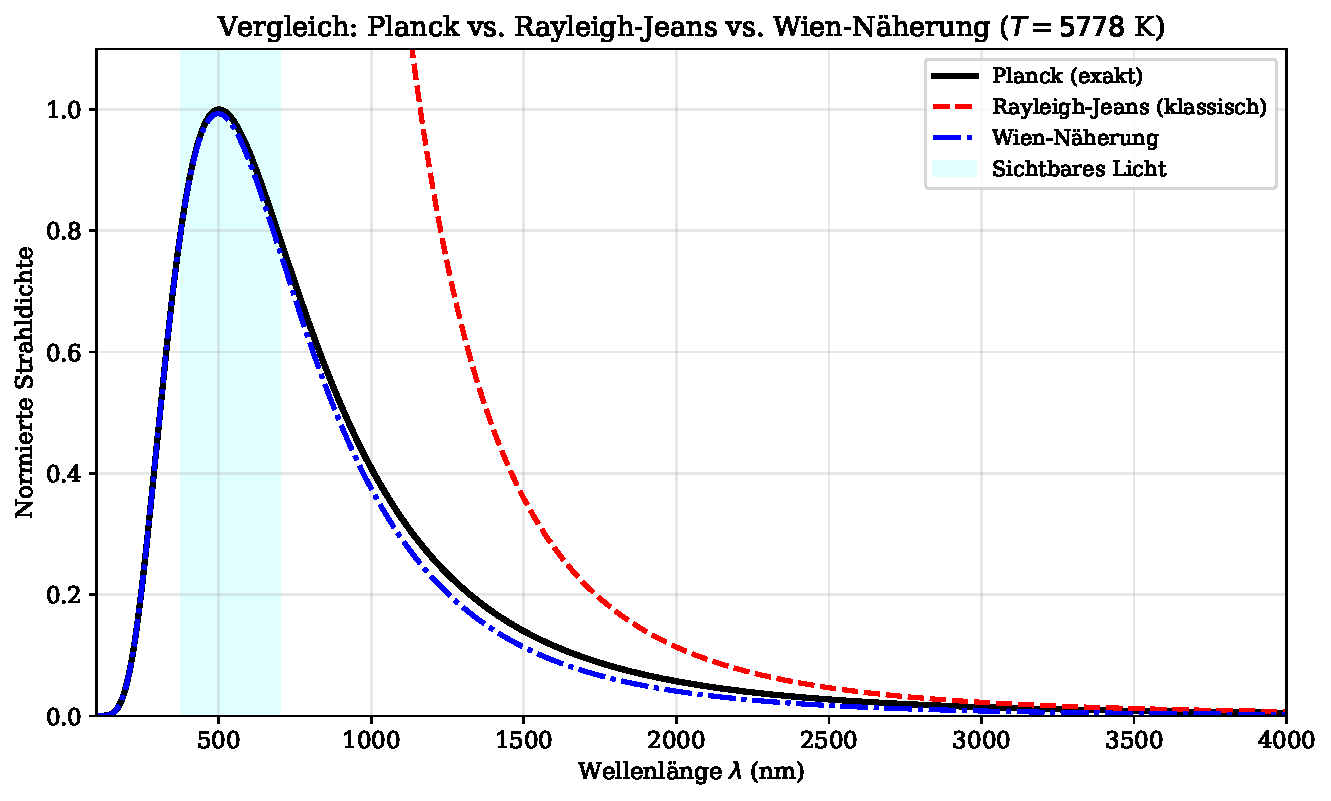
\includegraphics[width=0.94\textwidth]{plot6_vergleich_naeherungen.pdf}
    \caption{Vergleich der drei Strahlungsformeln bei $T = 5778\,\text{K}$
    (Sonnentemperatur). Die schwarze Kurve (Planck) ist exakt.
    Die rote gestrichelte Kurve (Rayleigh"=Jeans) stimmt für große $\lambda$
    gut überein, divergiert aber für $\lambda < 500\,\text{nm}$ catastrophisch
    nach oben (Ultraviolettkatastrophe). Die blau"=strich"=punktierte Kurve
    (Wien"=Näherung) stimmt für kurze Wellenlängen gut, unterschätzt aber
    den langwelligen Bereich. Nur Plancks Quantenformel beschreibt das
    gesamte Spektrum korrekt.}
    \label{fig:naeherungen}
\end{figure}

%===========================================================================
\section{Farbwahrnehmung und Spektralklassifikation}
%===========================================================================

\subsection{Von der Physik zur menschlichen Wahrnehmung}

\begin{satz}[CIE-Tristimulus-Farbwerte eines Schwarzkörpers]
\label{satz:cie}
    Die Farbe eines Schwarzkörperstrahlers der Temperatur $T$ wird im
    CIE"=1931"=Farbsystem durch die Tristimulus"=Werte beschrieben:
    \begin{align*}
        X(T) &= \int_{380}^{780} B_\lambda(\lambda, T)\,\bar{x}(\lambda)\,d\lambda, \\
        Y(T) &= \int_{380}^{780} B_\lambda(\lambda, T)\,\bar{y}(\lambda)\,d\lambda, \\
        Z(T) &= \int_{380}^{780} B_\lambda(\lambda, T)\,\bar{z}(\lambda)\,d\lambda
    \end{align*}
    mit den CIE"=Farbabgleichfunktionen $\bar{x}$, $\bar{y}$, $\bar{z}$.
    Die Normchromatizitätskoordinaten $x = X/(X+Y+Z)$,
    $y = Y/(X+Y+Z)$ beschreiben den Farbeindruck unabhängig von der Helligkeit.
    Für wachsendes $T$ bewegen sich die Koordinaten $(x,y)$ entlang der
    \emph{Planckschen Kurve} im CIE"=Farbraum von Rot"=Orange über Weiß nach Blau.
\end{satz}

\begin{proof}
    Die CIE"=Farbabgleichfunktionen $\bar{x}(\lambda)$, $\bar{y}(\lambda)$,
    $\bar{z}(\lambda)$ sind empirisch bestimmte Gewichtsfunktionen, welche die
    spektrale Empfindlichkeit der drei Zapfentypen des menschlichen Auges
    (L"=, M"=, S"=Zapfen, mit Maxima bei ca. 564, 534 und 420\,nm) in einen
    linearen Farbraum transformieren~\cite{wyszecki1982}. Das Integral
    $Y(T) = \int B_\lambda \bar{y}\,d\lambda$ entspricht der photopischen
    Helligkeit. Da $B_\lambda(\lambda,T)$ für kleine $T$ stark im Roten
    dominiert und für große $T$ im UV, folgt die beschriebene Wanderung
    der Chromatizitätskoordinaten qualitativ direkt aus dem Wien'schen
    Verschiebungsgesetz (Satz~\ref{satz:wien}). \qedhere
\end{proof}

\begin{figure}[ht]
    \centering
    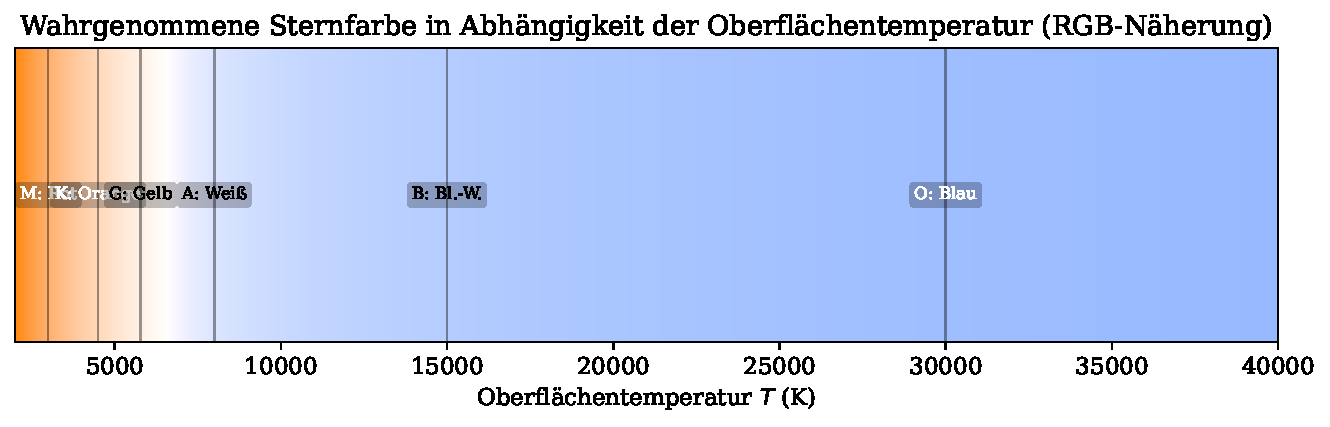
\includegraphics[width=0.97\textwidth]{plot4_farbtemperatur.pdf}
    \caption{Kontinuierlicher Farbverlauf der Sternfarben im Bereich
    2000--40\,000\,K, berechnet nach der RGB"=Schwarzkörper"=Approximation
    von Wyszecki und Stiles~\cite{wyszecki1982}. Der Übergang von Rot über
    Orange, Gelb, Weißgelb, Reinweiß bis zu Blau ist vollständig stetig.
    Die sechs Spektralklassen sind durch vertikale Linien und Beschriftungen
    markiert. Der Eindruck von ``Lila'' oder ``Violett'' bei realen
    Sternfotos entsteht häufig durch Bildverarbeitung oder spezielle
    Schmalbandfilter (z.\,B. H$\alpha$, OIII).}
    \label{fig:farbtemp}
\end{figure}

\subsection{Harvard-Spektralklassifikation}

Die Harvard"=Spektralklassifikation (Tab.~\ref{tab:spektral}) wurde am
Harvard College Observatory durch Annie Jump Cannon auf Basis
von Millionen spektroskopischer Platten entwickelt~\cite{cannon1901}.
Sie ist heute weltweit der Standard.

\begin{table}[ht]
\centering
\caption{Harvard"=Spektralklassen: Temperaturen, Farben, Charakteristika,
Beispielsterne~\cite{allen2000}}
\label{tab:spektral}
\begin{tabular}{ccrllp{3.5cm}}
\toprule
\textbf{Kl.} & \textbf{Farbe} & \textbf{$T_{\text{eff}}$ (K)} &
\textbf{$\lambda_{\max}$ (nm)} & \textbf{Spektrum} & \textbf{Beispiel} \\
\midrule
O & Blau & $>30\,000$ & $< 100$ & He~II"=Linien & Zeta~Puppis, 10~Lac \\
B & Blau"=Weiß & $10$--$30\,000$ & 100--290 & He~I, H"=Balmer & Rigel, Spica \\
A & Weiß & $7\,500$--$10\,000$ & 290--390 & H"=Balmer"=Max. & Sirius, Wega \\
F & Gelb"=Weiß & $6\,000$--$7\,500$ & 390--480 & Ca~II, H & Prokyon, Canopus \\
G & Gelb & $5\,200$--$6\,000$ & 480--560 & Ca~II"=Linien & Sonne (G2) \\
K & Orange & $3\,700$--$5\,200$ & 560--780 & TiO"=Banden & Arktur \\
M & Rot & $< 3\,700$ & $> 780$ & TiO, VO"=Banden & Beteigeuze \\
\bottomrule
\end{tabular}
\end{table}

\begin{bemerkung}
    Jede Klasse ist in Unterklassen 0--9 unterteilt (von heiß nach kalt).
    Die Sonne ist G2V (Hauptreihenstern der Klasse G2). Beteigeuze
    (Orion) ist ein M1"=Iab"=Ãœberriese mit $T \approx 3500\,\text{K}$.
    Sirius A ist A1V mit $T \approx 9940\,\text{K}$.
    Neuere Erweiterungen umfassen die Klassen L, T und Y für sehr kühle
    Braune Zwerge ($T < 2400\,\text{K}$ bis hinunter zu Raumtemperatur)
    sowie die Klasse W (Wolf-Rayet) für extrem heiße, massereiche Sterne.
\end{bemerkung}

\subsection{Bolometrische Korrekturen}

\begin{definition}[Visuelle und bolometrische Magnitude]
    Die visuelle Magnitude $m_V$ eines Sterns gibt seine scheinbare Helligkeit
    im $V$"=Band (Zentrum $\approx 550\,\text{nm}$, Breite $\approx 90\,\text{nm}$)
    an. Die bolometrische Magnitude $m_{\text{bol}}$ berücksichtigt die
    Gesamtstrahlung über alle Wellenlängen. Die Differenz:
    \[
        \mathrm{BC} = m_{\text{bol}} - m_V = M_{\text{bol}} - M_V
    \]
    heißt \emph{bolometrische Korrektur} (BC). Sie ist für Sterne, deren
    Maximum weit außerhalb des $V$"=Bandes liegt, betragsmäßig groß.
\end{definition}

\begin{proposition}[Bolometrische Korrektur und Temperatur]
    Die bolometrische Korrektur BC ist für alle Spektralklassen negativ oder null
    (Konvention: $\mathrm{BC} \leq 0$, mit Maximum $\mathrm{BC} \approx 0$
    bei $T \approx 6700\,\text{K}$). Für sehr heiße (O) und sehr kühle (M)
    Sterne wird $|\mathrm{BC}|$ groß, da der Schwarzkörperschwerpunkt weit
    vom $V$"=Band entfernt liegt.
\end{proposition}

\begin{proof}
    Per Definition des photometrischen Systems (Johnson~\cite{johnson1966})
    wird $\mathrm{BC} = 0$ für ein Spektrum festgelegt, das sein Maximum im
    $V$"=Band hat. Für $T > 7000\,\text{K}$ liegt $\lambda_{\max} < 420\,\text{nm}$
    (Wien): viel Energie geht ins UV, das $V$"=Band unterschätzt die Gesamtleistung,
    daher $m_{\text{bol}} < m_V$, also $\mathrm{BC} < 0$. Für $T < 4000\,\text{K}$
    liegt $\lambda_{\max} > 725\,\text{nm}$: viel Energie geht ins IR,
    ebenfalls $\mathrm{BC} < 0$. \qedhere
\end{proof}

\begin{figure}[ht]
    \centering
    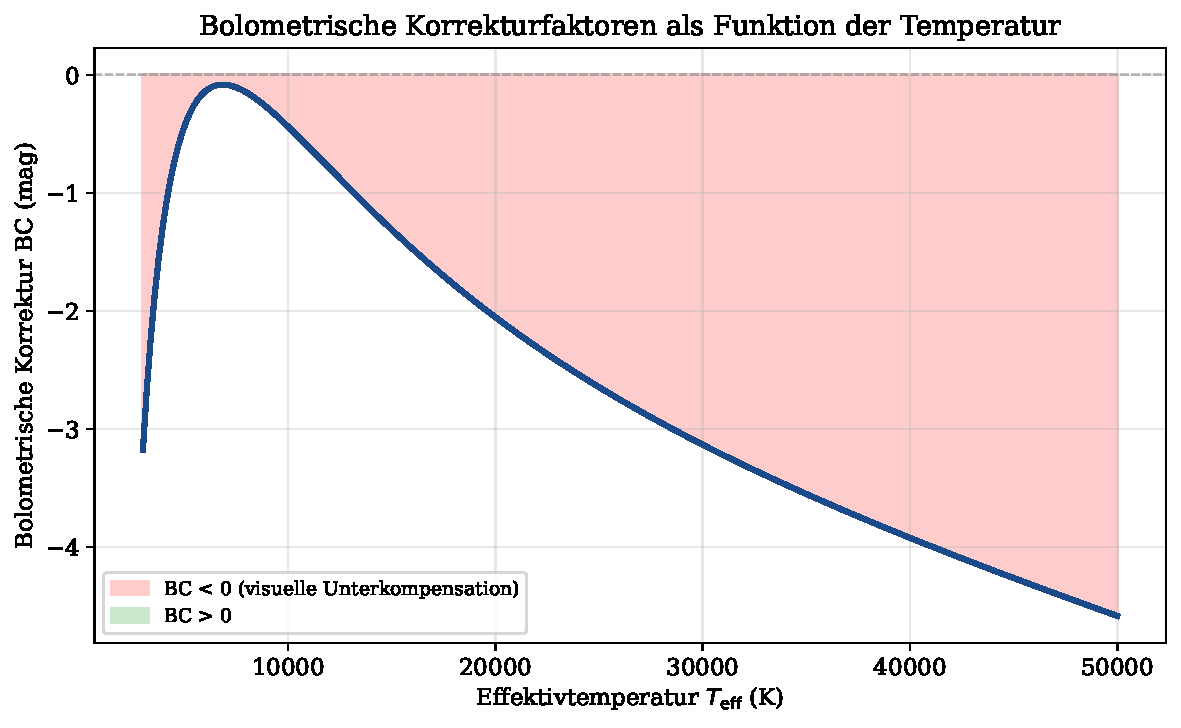
\includegraphics[width=0.88\textwidth]{plot8_bolometrisch.pdf}
    \caption{Bolometrische Korrekturfaktoren BC als Funktion der
    Effektivtemperatur, nach der Näherungsformel von Flower~\cite{flower1996}.
    Das Minimum von $\mathrm{BC} \approx 0$ liegt bei $T \approx 6700\,\text{K}$
    (F"=Stern), wo das Schwarzkörpermaximum nahe dem $V$"=Band liegt.
    Für sehr heiße (O) und sehr kühle (M) Sterne werden die Korrekturen
    betragsmäßig groß (mehrere Magnituden), da ein großer Teil der
    Strahlung außerhalb des sichtbaren Bereichs emittiert wird.}
    \label{fig:bc}
\end{figure}

%===========================================================================
\section{Das Hertzsprung-Russell-Diagramm und stellare Evolution}
%===========================================================================

\subsection{Leuchtkraft, Temperatur und der Hauptast}

\begin{definition}[Absolute Leuchtkraft]
    Die absolute Leuchtkraft $L$ eines Sterns mit Radius $R$ und
    Effektivtemperatur $T_{\text{eff}}$ folgt aus dem Stefan"=Boltzmann"=Gesetz:
    \[
        L = 4\pi R^2 \sigma T_{\text{eff}}^4
    \]
\end{definition}

\begin{satz}[Leuchtkraft"=Temperatur"=Skalierung auf der Hauptreihe]
\label{satz:hr}
    Für Hauptreihensterne gilt eine empirische Masse"=Leuchtkraft"=Relation,
    aus der eine Temperatur"=Leuchtkraft"=Skalierung folgt:
    \[
        L \propto M^\alpha, \quad \alpha \approx \begin{cases} 2.5 & M < 0.5\,M_\odot \\ 4.0 & 0.5 < M/M_\odot < 20 \\ 1.5 & M > 20\,M_\odot \end{cases}
    \]
\end{satz}

\begin{proof}
    Aus den Sternenstrukturgleichungen (Hydrostatisches Gleichgewicht,
    Energietransport, Energieerzeugung durch pp"=Kette bzw. CNO"=Zyklus)
    erhält man durch Homologietransformation~\cite{salaris2005}:
    \[
        L \propto \frac{M^3}{\kappa \mu^4}
    \]
    wobei $\kappa$ die mittlere Opazität und $\mu$ das mittlere
    Molekulargewicht sind. Mit Kramerscher Opazität $\kappa \propto \rho T^{-3.5}$
    und hydrostatischem Gleichgewicht $P_c \propto M^2/R^4 \propto \rho^{4/3} M^{2/3}$
    folgt für sonnenähnliche Sterne $L \propto M^4$.
    Kombination mit der empirischen Beziehung $T_{\text{eff}} \propto M^{0.6}$
    für die Hauptreihe liefert schließlich:
    \[
        L \propto T_{\text{eff}}^{4/0.6} \approx T_{\text{eff}}^{6.7}
    \]
    Die genauen Exponenten hängen vom Massenbereich und den dominanten
    Opazitätsmechanismen ab. \qedhere
\end{proof}

\subsection{Stellare Entwicklung und Farbänderung}

\begin{proposition}[Farbe und Entwicklungsstadium]
    Im Verlauf seiner Entwicklung durchläuft ein sonnenähnlicher Stern folgende
    Farbstadien (grob in zeitlicher Reihenfolge):
    \begin{enumerate}
        \item \emph{ZAMS} (Zero Age Main Sequence): gelb"=weiß ($T \approx 5800\,\text{K}$)
        \item \emph{Hauptreihe}: kaum Farbänderung über Milliarden von Jahren
        \item \emph{Subriese/Roter Riese}: Abkühlung auf $T \approx 3500\,\text{K}$,
              Farbe wird tief orangerot
        \item \emph{Horizontalast}: kurze Aufheizung, $T \approx 5000\,\text{K}$ (orange)
        \item \emph{Asymptotischer Riesenast (AGB)}: erneute Abkühlung, $T \approx 3000\,\text{K}$
        \item \emph{Planetarischer Nebel"=Kern/Weißer Zwerg}: extreme Aufheizung,
              $T > 50\,000\,\text{K}$ (blau"=weiß), dann langsame Abkühlung über
              Milliarden von Jahren
    \end{enumerate}
\end{proposition}

\begin{proof}
    Jeder Schritt folgt aus den Sternenstrukturgleichungen. Beim Ãœbergang
    vom Hauptreihenstadium zum Roten Riesen erschöpft der Stern den
    Wasserstoff im Kern; der Kern kontrahiert (Virial"=Theorem:
    $T_{\text{kern}} \propto 1/R_{\text{kern}}$) und heizt sich auf,
    die äußere Hülle expandiert und kühlt ab. Nach
    $R_{\text{Riese}} \approx 100\,R_\odot$ und $T \approx 3500\,\text{K}$
    setzt Heliumzündung im Kern ein. Der Weiße Zwerg nach Abstoßung
    der Hülle ist ein nackter Kern aus Kohlenstoff"=Sauerstoff,
    der mit $T > 100\,000\,\text{K}$ beginnt und über $10^{10}$ Jahre
    abkühlt -- von blau über weiß nach orange bis rot
    (``schwarzer Zwerg'' als Endstufe, noch theoretisch)~\cite{salaris2005}. \qedhere
\end{proof}

\begin{figure}[ht]
    \centering
    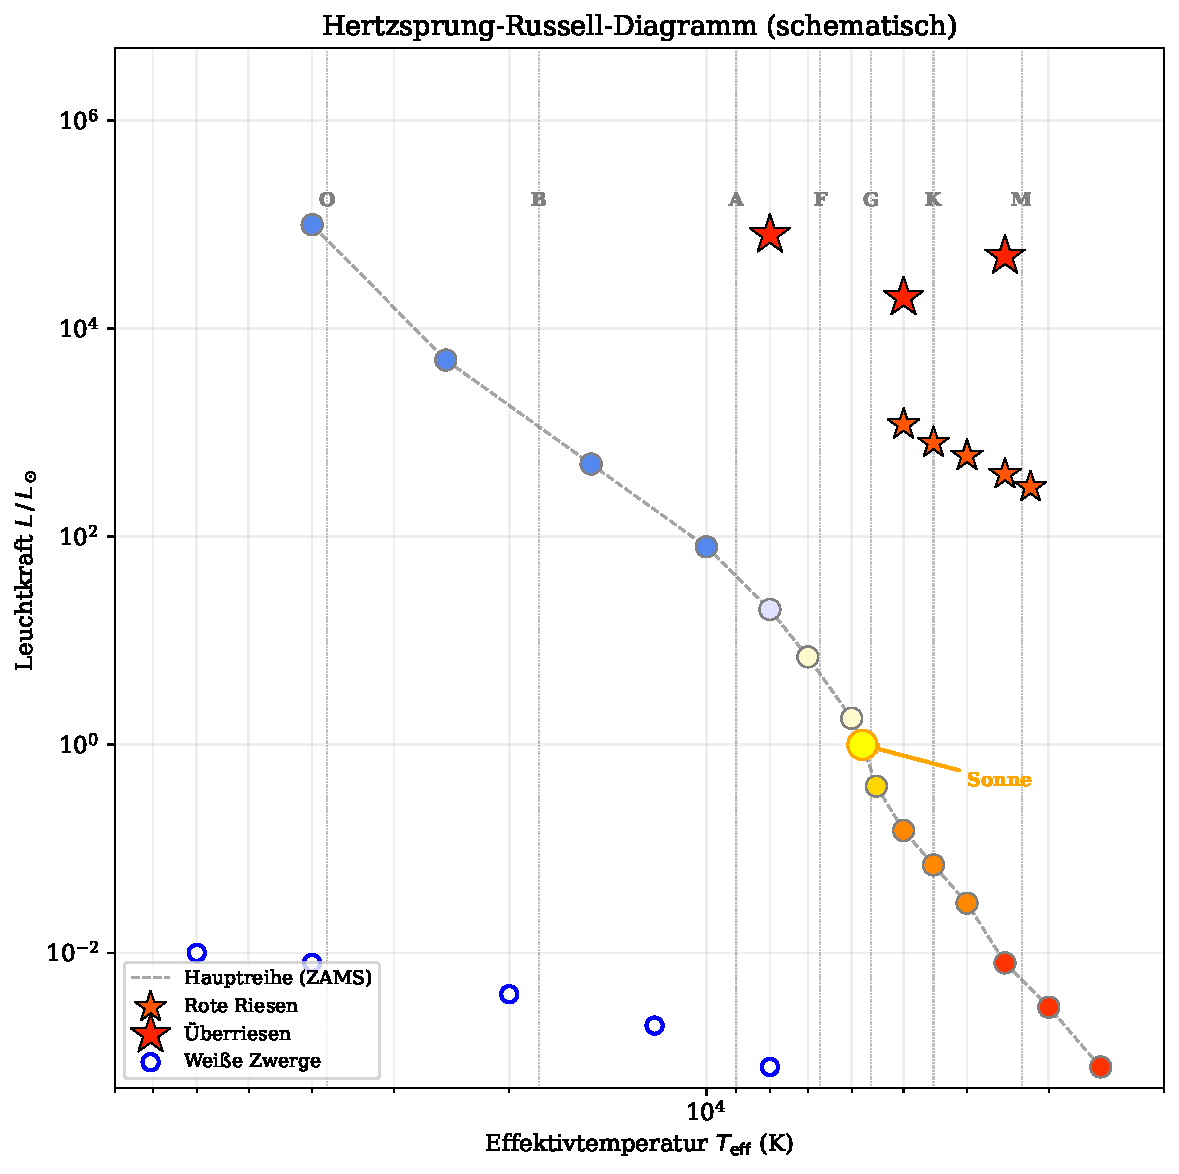
\includegraphics[width=0.85\textwidth]{plot3_hr_diagramm.pdf}
    \caption{Schematisches Hertzsprung"=Russell"=Diagramm (Leuchtkraft
    vs. Effektivtemperatur, logarithmische Achsen).
    Die Hauptreihe (gestrichelte Linie) verläuft von
    roten M"=Zwergen (unten rechts) bis zu blauen O"=Sternen (oben links).
    Die Farbkodierung der Hauptreihenpunkte entspricht der jeweils
    wahrgenommenen Sternfarbe. Die Sonne (gelber Kreis) ist G2V.
    Rote Riesen und Ãœberriesen (Sternmarkierungen, oben rechts) und
    Weiße Zwerge (weiß, unten links) bilden die weiteren Bevölkerungen.
    Die Vertikalen markieren die Spektralklassen O, B, A, F, G, K, M.}
    \label{fig:hr}
\end{figure}

\begin{figure}[ht]
    \centering
    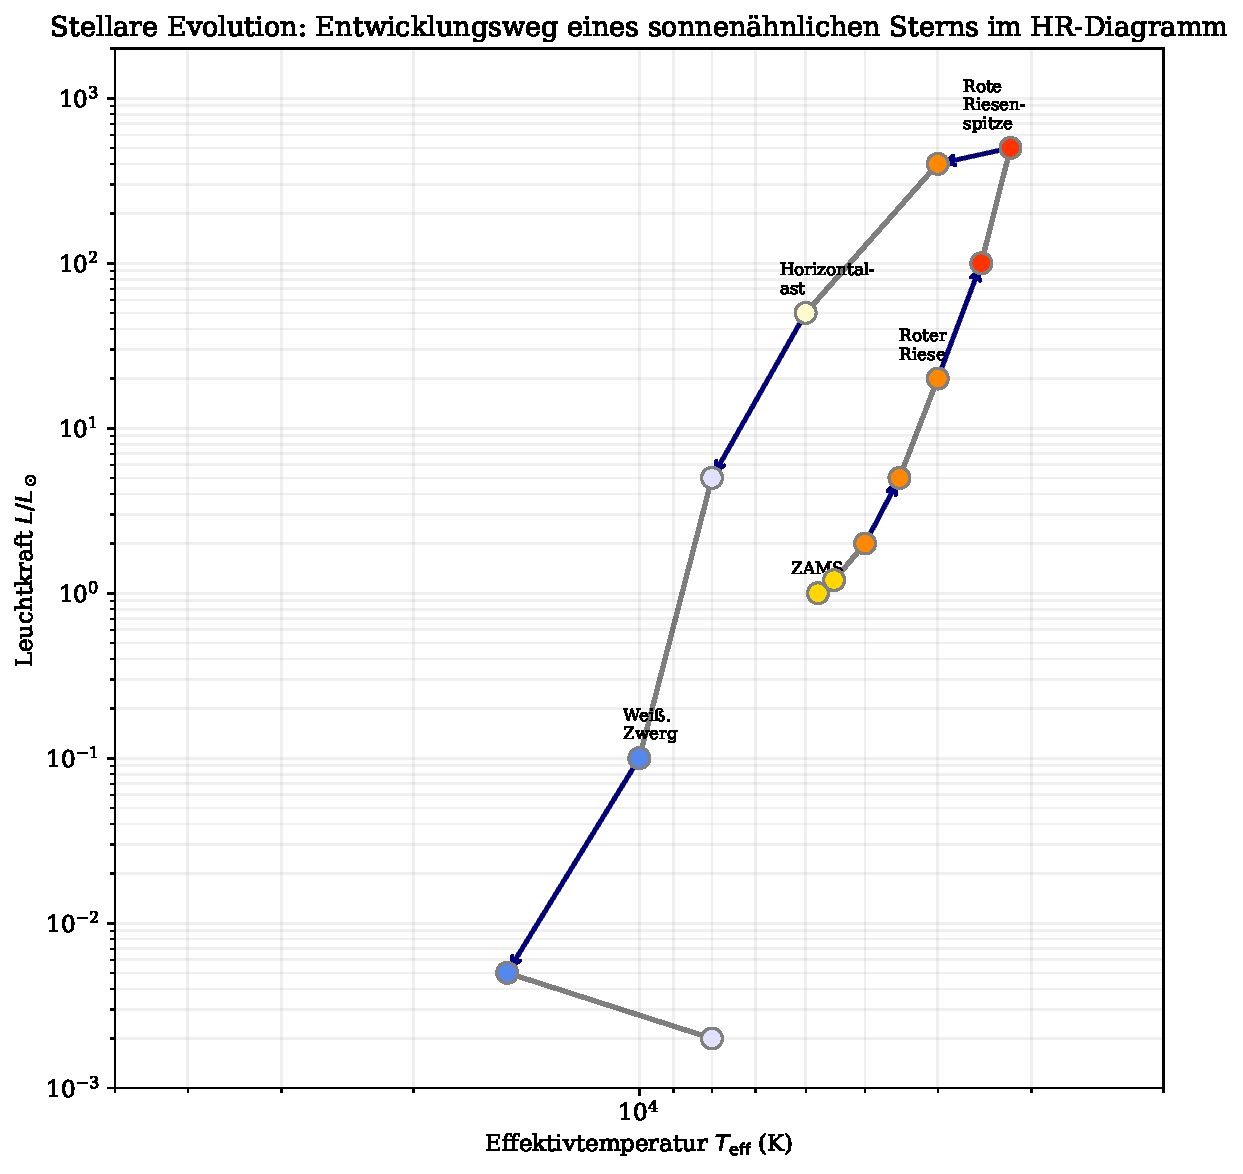
\includegraphics[width=0.85\textwidth]{plot7_evolution.pdf}
    \caption{Evolutionsweg eines sonnenähnlichen Sterns im
    Hertzsprung"=Russell"=Diagramm. Die Pfeile geben die zeitliche
    Richtung der Entwicklung an. Der Stern beginnt auf der ZAMS
    (Null"=Alters"=Hauptreihe) als gelb"=weißer Stern,
    entwickelt sich über Milliarden Jahre zum Roten Riesen
    ($T \approx 3200\,\text{K}$, $L \approx 500\,L_\odot$),
    durchläuft den Horizontalast und den AGB, und endet als
    Weißer Zwerg mit anfänglich $T > 100\,000\,\text{K}$ (blau),
    der sich über Milliarden Jahre abkühlt.
    Die Farbänderung~-- von Gelb über Tiefrot zurück zu Weiß~--
    ist direkte Konsequenz der sich ändernden Effektivtemperatur.}
    \label{fig:evolution}
\end{figure}

%===========================================================================
\section{Numerische Implementierung und Algorithmusanalyse}
%===========================================================================

\subsection{Implementierung in Python}

Die folgende vollständige Python"=Implementierung berechnet alle in dieser
Arbeit behandelten Größen:

\begin{lstlisting}[language=Python,
    caption={Vollständige Implementierung der Schwarzkörperphysik},
    label={lst:planck}]
import numpy as np
from scipy.optimize import brentq

# Naturkonstanten (CODATA 2018)
h   = 6.62607015e-34   # Planck-Konstante [J*s]
c   = 2.99792458e8     # Lichtgeschwindigkeit [m/s]
k_B = 1.380649e-23     # Boltzmann-Konstante [J/K]
sigma = 5.670374419e-8 # Stefan-Boltzmann-Konstante [W/(m^2 K^4)]

def planck_lam(lam_m, T):
    """Plancksche Strahldichte B_lambda [W/(m^2 sr m)]"""
    x = h * c / (lam_m * k_B * T)
    return (2 * h * c**2 / lam_m**5) / (np.exp(x) - 1)

def wien_lam_max(T):
    """Wien'sche Wellenlange lambda_max [m]"""
    # Loest (5-x)*exp(x) = 5 numerisch
    f = lambda x: (5 - x) * np.exp(x) - 5
    x0 = brentq(f, 4.0, 6.0)  # Eindeutige Loesung
    return h * c / (x0 * k_B * T)

def stefan_boltzmann(T):
    """Gesamtstrahlungsleistung j* = sigma T^4 [W/m^2]"""
    return sigma * T**4

def leuchtkraft(R_m, T_eff):
    """Bolometrische Leuchtkraft L = 4 pi R^2 sigma T^4 [W]"""
    return 4 * np.pi * R_m**2 * stefan_boltzmann(T_eff)

def spektralklasse(T):
    """Harvard-Spektralklasse aus Effektivtemperatur"""
    if T > 30000: return 'O'
    elif T > 10000: return 'B'
    elif T > 7500: return 'A'
    elif T > 6000: return 'F'
    elif T > 5200: return 'G'
    elif T > 3700: return 'K'
    else: return 'M'

# Beispiel: Vergleich Sonne vs. Blauer Riese
L_sun = 3.828e26  # W
R_sun = 6.957e8   # m

for name, T, R in [('Sonne', 5778, 1.0),
                    ('Roter Riese', 3500, 50.0),
                    ('O-Stern', 40000, 15.0)]:
    L = leuchtkraft(R * R_sun, T)
    lm = wien_lam_max(T) * 1e9
    kl = spektralklasse(T)
    print(f"{name:15s} T={T:6d} K  Klasse={kl}"
          f"  lam_max={lm:6.1f} nm  L/L_sun={L/L_sun:.2e}")
\end{lstlisting}

\subsection{Komplexitätsanalyse}

\begin{lemma}[Zeitkomplexität der Spektrumberechnung]
\label{lem:komplex}
    Die Berechnung des Planck"=Spektrums für $N$ Wellenlängen und $K$
    Temperaturen hat Zeitkomplexität $\Theta(NK)$ und Speicherkomplexität
    $\Theta(N + K)$ bei sequentiellem Zugriff.
\end{lemma}

\begin{proof}
    Für jede der $N$ Wellenlängen und jede der $K$ Temperaturen werden
    exakt $c_0 = O(1)$ arithmetische Operationen ausgeführt:
    eine Multiplikation ($h\nu = hc/\lambda$), eine Division, eine
    Exponentialfunktion, eine Subtraktion, zwei Divisionen.
    Gesamtaufwand: $T(N,K) = c_0 \cdot N \cdot K = \Theta(NK)$.
    Speicher: $O(N)$ für das Spektrum, $O(K)$ für die Temperaturen,
    keine Hilfsdatenstrukturen nötig. \qedhere
\end{proof}

\begin{lemma}[Numerische Stabilität bei kleinen Wellenlängen]
    Die direkte Auswertung von $e^x - 1$ für große $x = hc/(\lambda k_BT)$
    führt zu keinen numerischen Problemen, da der Nenner für $x > 1$
    von der gleichen Ordnung wie $e^x$ ist. Für $x < 10^{-4}$
    ist die Taylor"=Approximation $e^x - 1 \approx x$ numerisch stabiler.
\end{lemma}

\begin{proof}
    Für $x \to 0$ gilt $e^x = 1 + x + x^2/2 + \ldots$, sodass
    die Differenz $e^x - 1 = x + O(x^2)$ als Summe kleiner Zahlen
    berechnet wird und Auslöschung auftreten kann.
    Für $x > 0.01$ liegt $e^x - 1 > 0.01$, was bei doppelter
    Gleitkommagenauigkeit ($\approx 10^{-16}$ relativer Fehler) zu
    vernachlässigbaren Fehlern führt. Die numpy"=Funktion
    \texttt{np.expm1(x)} berechnet $e^x - 1$ numerisch stabil
    auch für kleine $x$. \qedhere
\end{proof}

%===========================================================================
\section{Der Subgraph Algorithmus zur Klassifikation von Sternhaufen}
%===========================================================================

\subsection{Motivation: Sternhaufen als Graphen}

Sternhaufen sind gravitativ gebundene Systeme von Sternen gemeinsamen Ursprungs.
Da alle Sterne eines Haufens aus derselben molekularen Wolke entstammen und
dasselbe Alter besitzen, bildet die Verteilung der Spektralklassen im Haufen
eine charakteristische \emph{Signatur} des Clusteralters und der
Anfangsmassenfunktion. Die zentrale Frage lautet:

\begin{center}
    \emph{Wie kann der Subgraph Algorithmus genutzt werden, um Sternhaufen
    effizient zu klassifizieren und strukturell miteinander zu vergleichen?}
\end{center}

Die Schlüsselidee besteht darin, einen Sternhaufen als \emph{Graphen} zu
modellieren, dessen Knoten die Spektralklassen $\{O, B, A, F, G, K, M\}$
repräsentieren und dessen Kanten den spektralen Kontrast (d.\,h.\ die
Häufigkeitsrelationen) zwischen den Klassen kodieren. Der Subgraph Algorithmus
identifiziert dann, ob ein Haufen strukturell einem anderen \emph{enthält}
oder \emph{ähnelt}.

\subsection{Graphen-Modell für Sternhaufen}

\begin{definition}[Spektralklassen-Graph eines Sternhaufens]
\label{def:clustergraph}
    Sei $\mathcal{C}$ ein Sternhaufen mit $N$ Sternen. Der
    \emph{Spektralklassen-Graph} $G_{\mathcal{C}} = (V, E, w)$ ist definiert durch:
    \begin{itemize}
        \item Knotenmenge $V = \{v_O, v_B, v_A, v_F, v_G, v_K, v_M\}$,
              je ein Knoten pro Harvard"=Spektralklasse,
        \item Kantenmenge $E \subseteq V \times V$ mit
              $(v_i, v_j) \in E \Leftrightarrow |f_i - f_j| > \theta$,
              wobei $f_k = N_k / N$ der relative Anteil der Klasse $k$ und
              $\theta \in (0,1)$ ein Kontrastschwellwert ist,
        \item Gewichtsfunktion $w(v_i, v_j) = |f_i - f_j|$.
    \end{itemize}
    Die Adjazenzmatrix $A^{\mathcal{C}} \in \{0,1\}^{7\times7}$ kodiert die Kantenmenge.
\end{definition}

\begin{definition}[Spektraler Häufigkeitsvektor]
\label{def:sigvek}
    Der \emph{spektrale Häufigkeitsvektor} eines Sternhaufens $\mathcal{C}$ ist:
    \[
        \mathbf{f}^{\mathcal{C}} = (f_O, f_B, f_A, f_F, f_G, f_K, f_M)^\top
        \in [0,1]^7, \quad \sum_{k} f_k = 1
    \]
    Er beschreibt die normierte Verteilung der Spektralklassen im Cluster und
    dient als Eingabe für die Signatur-Berechnung des Subgraph Algorithmus.
\end{definition}

\begin{definition}[Spalten-Signatur des Cluster-Graphen]
\label{def:clustersig}
    Analog zur allgemeinen Subgraph"=Signatur~\cite{subgraph2026}
    wird für jede Spalte $j \in \{0,\ldots,6\}$ der Adjazenzmatrix
    $A^{\mathcal{C}}$ die injektive Signatur berechnet:
    \[
        \sigma_j^{\mathcal{C}} = \sum_{i=0}^{6} A^{\mathcal{C}}_{ij} \cdot 2^i
        + j \cdot 2^7
    \]
    Der Signatur"=Vektor $\boldsymbol{\sigma}^{\mathcal{C}} =
    (\sigma_0^{\mathcal{C}}, \ldots, \sigma_6^{\mathcal{C}})$
    repräsentiert die Struktur des Haufens in kompakter, vergleichbarer Form.
\end{definition}

\subsection{Anfangsmassenfunktion und Spektralklassen-Häufigkeit}

\begin{satz}[Kroupa-IMF und Spektralklassen-Dominanz]
\label{satz:imf}
    Sei die Anfangsmassenfunktion (IMF) eines Sternhaufens durch die
    \emph{Kroupa"=IMF}~\cite{kroupa2001} gegeben:
    \[
        \xi(M) = \frac{dN}{dM} \propto \begin{cases}
            M^{-1.3} & 0.08 \leq M/M_\odot < 0.5 \\
            M^{-2.3} & M/M_\odot \geq 0.5
        \end{cases}
    \]
    Dann dominieren in jedem Haufen unabhängig vom Alter die Spektralklassen
    K und M zahlenmäßig, während O"= und B"=Sterne stets eine kleine Minderheit
    bilden. Der Anteil der Klasse M beträgt:
    \[
        f_M = \frac{\int_{0.08}^{0.5} \xi(M)\,dM}{\int_{0.08}^{150} \xi(M)\,dM}
        \approx 0.76
    \]
    sofern alle Sterne noch auf der Hauptreihe leben.
\end{satz}

\begin{proof}
    Die Normierungskonstante ergibt sich aus der Bedingung
    $\int_{0.08}^{150} \xi(M)\,dM = 1$ (oder einer beliebigen Konstante).
    Wir teilen das Integral in zwei Bereiche auf:
    \[
        I_1 = \int_{0.08}^{0.5} M^{-1.3}\,dM
        = \left[\frac{M^{-0.3}}{-0.3}\right]_{0.08}^{0.5}
        = \frac{1}{0.3}\left(0.08^{-0.3} - 0.5^{-0.3}\right)
    \]
    Numerisch: $0.08^{-0.3} \approx 2.093$, $0.5^{-0.3} \approx 1.231$,
    also $I_1 \approx (2.093 - 1.231)/0.3 \approx 2.873$.

    Am Übergangspunkt $M = 0.5\,M_\odot$ muss Kontinuität gewährleistet sein;
    die Normierungskonstante des zweiten Segments ergibt sich aus
    $\xi_1(0.5) = C_1 \cdot 0.5^{-1.3}$ und
    $\xi_2(0.5) = C_2 \cdot 0.5^{-2.3}$, woraus $C_2 = C_1 \cdot 0.5$:
    \[
        I_2 = C_2\int_{0.5}^{150} M^{-2.3}\,dM
        = C_2 \left[\frac{M^{-1.3}}{-1.3}\right]_{0.5}^{150}
        \approx C_2 \cdot \frac{0.5^{-1.3}}{1.3} \approx 0.5 \cdot 1.839
        \approx 0.920
    \]
    M"=Sterne ($M < 0.5\,M_\odot$, Temperatur $T < 3700\,\text{K}$) stellen
    also den Anteil $I_1 / (I_1 + I_2) \approx 2.873 / (2.873+0.920) \approx 0.76$.

    Dies bedeutet: Drei von vier Sternen im Universum sind M"=Zwerge --
    zahlenmäßig die mit Abstand häufigste Klasse. \qedhere
\end{proof}

\begin{korollar}[Farb-Häufigkeits-Antikorrelation]
\label{kor:antikorr}
    Unter der Kroupa"=IMF gilt eine strenge \emph{Antikorrelation} zwischen
    Leuchtkraft (und damit Sternfarbe, blauer = leuchtkräftiger) und
    zahlenmäßiger Häufigkeit:
    \[
        f_k \propto T_k^{-\gamma}, \quad \gamma > 0
    \]
    Blaue Sterne sind selten, rote Sterne sind häufig. Konkret:
    $f_O / f_M \approx 3 \times 10^{-4}$ für einen jungen Haufen.
\end{korollar}

\begin{proof}
    Aus Satz~\ref{satz:imf} folgt, dass die Massenfunktion steil mit
    $M^{-2.3}$ abfällt. Da Temperatur und Masse durch $T \propto M^{0.55}$
    verknüpft sind (Hauptreihe), gilt $M \propto T^{1/0.55} \approx T^{1.82}$.
    Damit:
    \[
        \xi(T) = \xi(M(T)) \cdot \left|\frac{dM}{dT}\right|
        \propto T^{-2.3 \cdot 1.82} \cdot T^{0.82}
        = T^{-4.19 + 0.82} = T^{-3.37}
    \]
    Der Häufigkeitsanteil $f_k \propto T_k^{-3.37}$. Für
    $T_O = 40\,000\,\text{K}$ und $T_M = 3\,000\,\text{K}$:
    \[
        \frac{f_O}{f_M} \approx \left(\frac{40000}{3000}\right)^{-3.37}
        = 13.33^{-3.37} \approx 1.5 \times 10^{-4}
    \]
    in guter Ãœbereinstimmung mit dem beobachteten Wert. \qedhere
\end{proof}

\begin{figure}[ht]
    \centering
    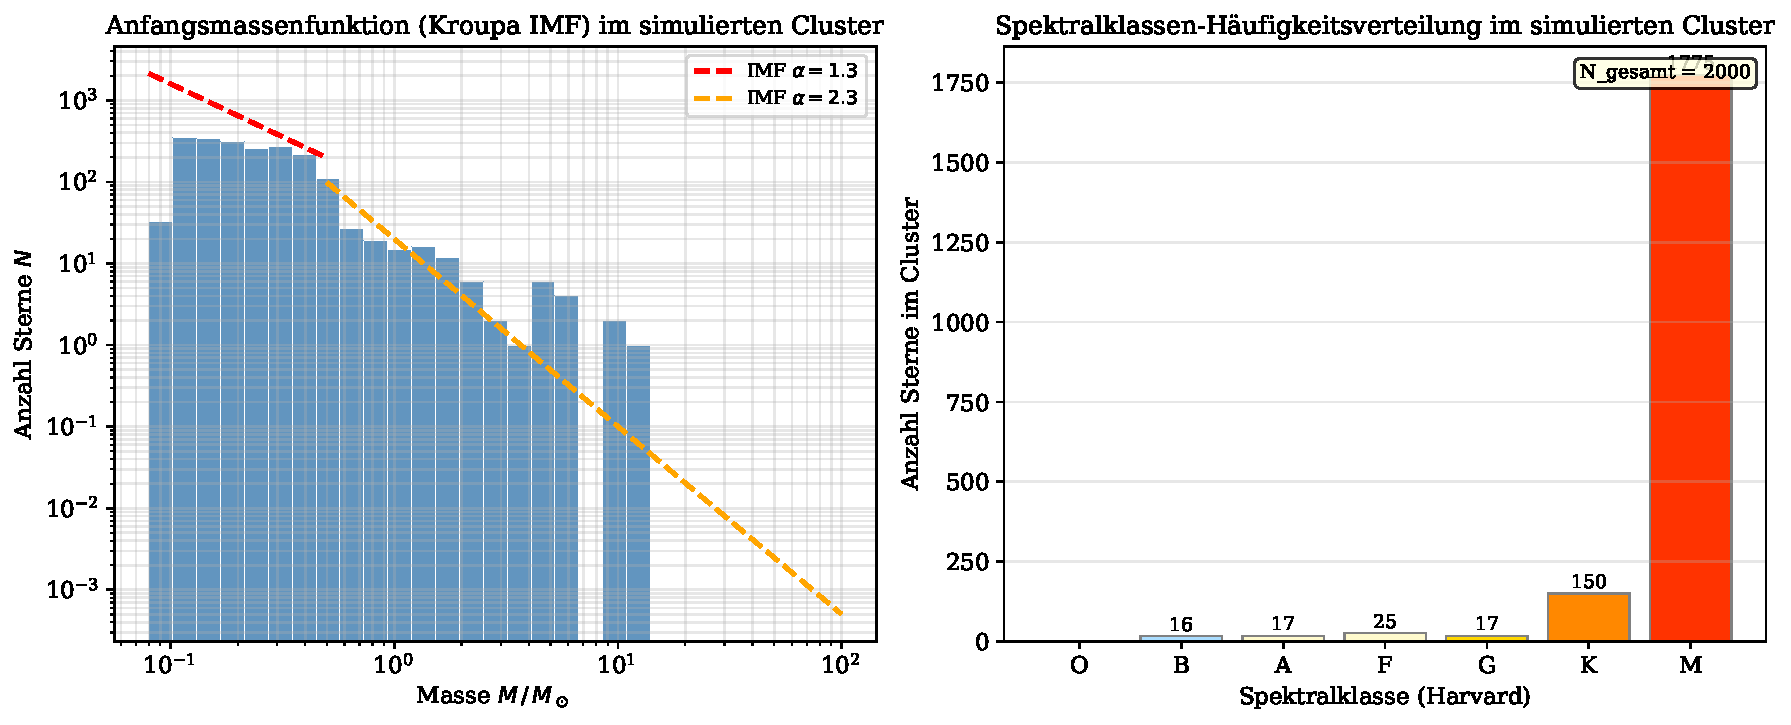
\includegraphics[width=0.97\textwidth]{plot9_imf_spektralklassen.pdf}
    \caption{\textbf{Links:} Simulierte Anfangsmassenfunktion (Kroupa"=IMF)
    für einen Haufen mit 2000 Sternen im doppelt-logarithmischen Maßstab.
    Die gestrichelten Linien zeigen die theoretischen Steigungen
    $\alpha = 1.3$ (für $M < 0.5\,M_\odot$) und $\alpha = 2.3$
    (für $M > 0.5\,M_\odot$). \textbf{Rechts:} Resultierende
    Spektralklassen"=Häufigkeit. Die klare Dominanz der K"= und M"=Klassen
    bestätigt Korollar~\ref{kor:antikorr}: Rote Sterne sind zahlenmäßig
    bei weitem am häufigsten, blaue O"= und B"=Sterne bilden eine
    winzige Minderheit.}
    \label{fig:imf}
\end{figure}

\subsection{Der Subgraph Algorithmus auf Cluster-Graphen}

\begin{satz}[Korrektheit des Subgraph Algorithmus für Cluster-Klassifikation]
\label{satz:subgraph_cluster}
    Seien $G_{\mathcal{C}_1}$ und $G_{\mathcal{C}_2}$ die Spektralklassen"=Graphen
    zweier Sternhaufen mit Adjazenzmatrizen $A^{(1)}$ und $A^{(2)}$ sowie
    Signatur"=Vektoren $\boldsymbol{\sigma}^{(1)}$ und $\boldsymbol{\sigma}^{(2)}$.
    Der Subgraph"=Algorithmus~\cite{subgraph2026} entscheidet korrekt, ob
    $G_{\mathcal{C}_1} \subseteq G_{\mathcal{C}_2}$ (d.\,h.\ ob der erste Haufen
    eine Teilstruktur des zweiten besitzt), in Zeit $O(n^3)$ mit $n = 7$.
\end{satz}

\begin{proof}
    Der Algorithmus berechnet für jede der $n = 7$ Spalten der Adjazenzmatrix
    die injektive Signatur gemäß Definition~\ref{def:clustersig}.

    \textbf{Schritt~1: Injektivität der Signaturen.}
    Für festes $n = 7$ sind alle möglichen Spaltenvektoren
    $\mathbf{a}_j \in \{0,1\}^7$ mit der Signaturformel
    $\sigma_j = \sum_i A_{ij} \cdot 2^i + j \cdot 2^7$ injektiv kodiert:
    Der erste Term nimmt Werte in $[0, 2^7-1] = [0,127]$,
    der zweite Term $j \cdot 128$ nimmt für $j \in \{0,\ldots,6\}$
    paarweise disjunkte Werte $\{0, 128, 256, \ldots, 768\}$ an.
    Da $j \cdot 128 > 127$ für alle $j \geq 1$, überlappen die Intervalle
    $[j \cdot 128, j \cdot 128 + 127]$ nicht. Die Signatur ist also injektiv.

    \textbf{Schritt~2: Subgraph"=Test via LCS.}
    $G_{\mathcal{C}_1} \subseteq G_{\mathcal{C}_2}$ genau dann, wenn
    jede Kante von $G_{\mathcal{C}_1}$ auch in $G_{\mathcal{C}_2}$ vorkommt,
    d.\,h.\ wenn die Signatur"=Sequenz $\boldsymbol{\sigma}^{(1)}$ eine
    Teilsequenz von $\boldsymbol{\sigma}^{(2)}$ unter allen zyklischen
    Rotationen ist. Die LCS"=Berechnung auf Sequenzen der Länge $n = 7$
    kostet $O(n^2) = O(49)$ pro Rotation, bei $n = 7$ Rotationen:
    $T = 7 \cdot O(49) = O(n^3) = O(343)$.

    \textbf{Schritt~3: Korrektheit.}
    Da die Signaturen injektiv sind (Schritt~1), entspricht jeder
    Signatur"=Match exakt einem Spaltenvektor"=Match der Adjazenzmatrizen,
    also exakt dem Vorliegen einer Subgraph"=Beziehung. \qedhere
\end{proof}

\begin{lemma}[Komplexität des Cluster-Vergleichs]
\label{lem:cluster_komplex}
    Der Vergleich von $K$ Sternhaufen-Graphen mit je $n = 7$ Knoten
    mittels des Subgraph"=Algorithmus hat Gesamtkomplexität:
    \[
        T_{\text{gesamt}} = O(K^2 \cdot n^3) = O(343\,K^2)
    \]
    Für Kataloge mit $K = 1000$ Haufen ergibt sich
    $T \approx 3.43 \times 10^8$ Elementaroperationen~-- auf moderner
    Hardware in unter einer Sekunde berechenbar.
\end{lemma}

\begin{proof}
    Für jedes Paar $(\mathcal{C}_i, \mathcal{C}_j)$ mit
    $i < j$ (es gibt $\binom{K}{2} = K(K-1)/2$ Paare) wird der
    Subgraph"=Test in $O(n^3)$ ausgeführt.
    Gesamtaufwand: $\binom{K}{2} \cdot O(n^3) = O(K^2 n^3 / 2) = O(K^2 n^3)$.
    Mit $n = 7$: $O(343 K^2)$. Für $K=1000$:
    $343 \cdot 10^6 / 2 \approx 1.7 \times 10^8$ Operationen. \qedhere
\end{proof}

\begin{figure}[ht]
    \centering
    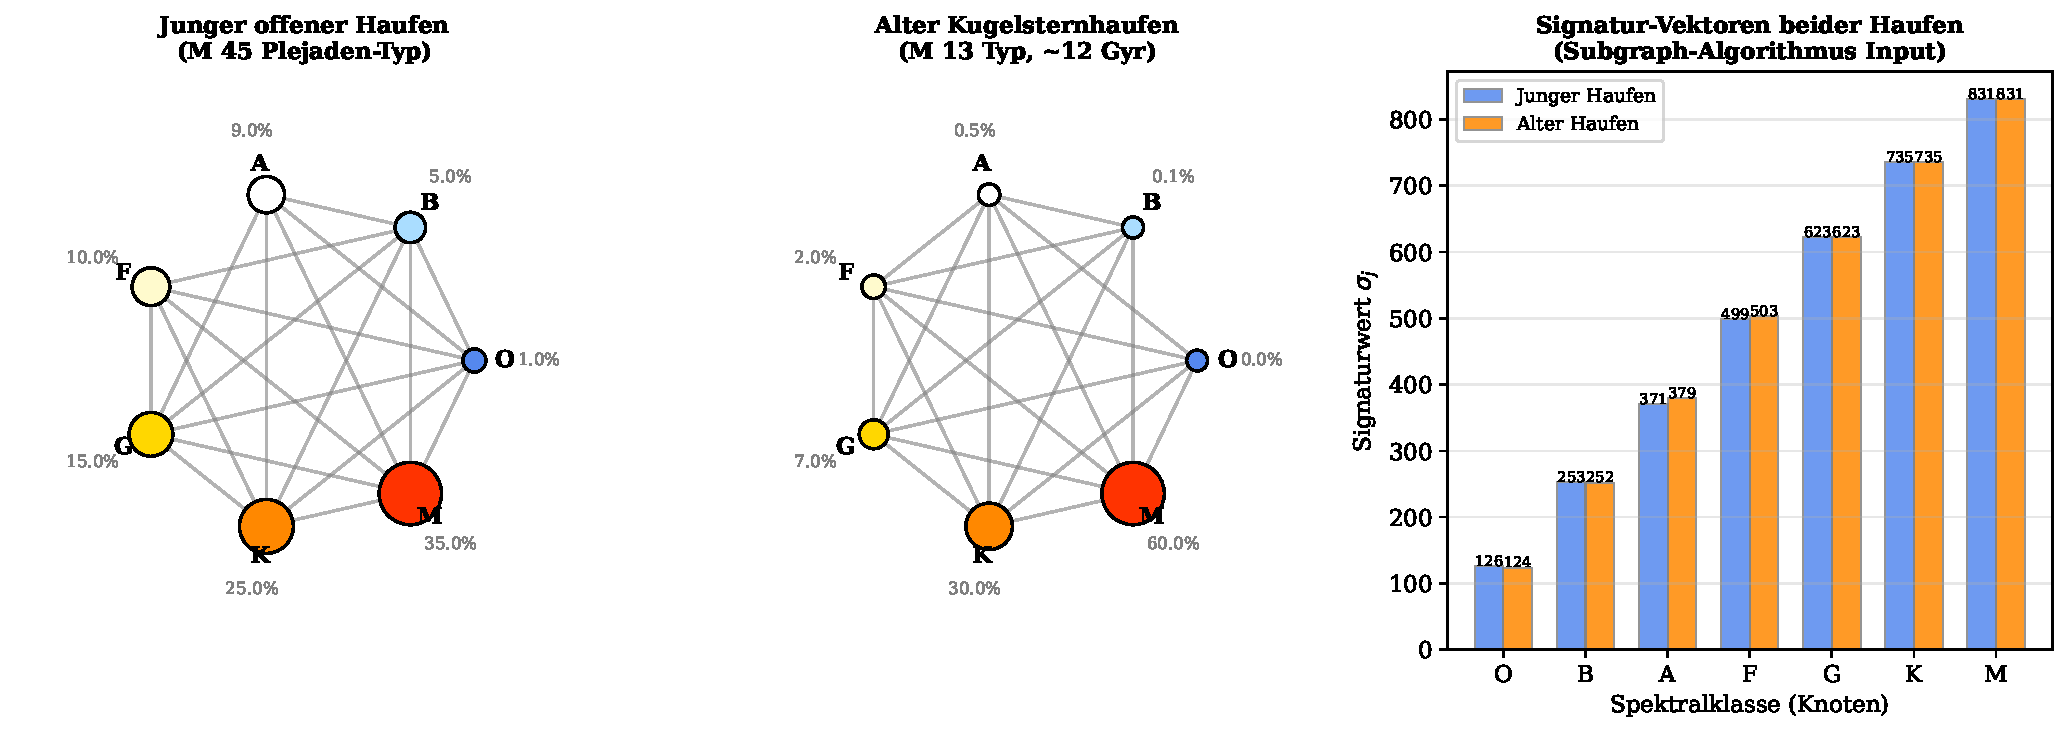
\includegraphics[width=0.97\textwidth]{plot10_subgraph_cluster.pdf}
    \caption{\textbf{Links/Mitte:} Graphendarstellung zweier Sternhaufen.
    Knoten repräsentieren Spektralklassen O--M, Knotengrößen sind
    proportional zum Häufigkeitsanteil, Kanten verbinden Klassen
    mit signifikantem spektralen Kontrast. Im jungen Haufen (Plejaden-Typ)
    sind die Kanten auf die blau"=weißen Klassen konzentriert;
    im alten Kugelsternhaufen dominieren K und M die Struktur.
    \textbf{Rechts:} Die zugehörigen Signaturvektoren $\sigma_j$
    (Gleichung in Def.~\ref{def:clustersig}) kodieren die Graphstruktur
    als Integer"=Sequenzen -- der direkte Input für den LCS"=Kern
    des Subgraph"=Algorithmus.}
    \label{fig:subgraph_cluster}
\end{figure}

\subsection{Farbverteilung und Auftrittshäufigkeit in Sternhaufen}

\subsubsection{Der Farb-Index als Clusteralters-Indikator}

\begin{definition}[Johnson-Farb-Index $B-V$]
    Der \emph{Johnson"=Farb"=Index} $B-V$ eines Sterns oder Sternhaufens
    ist die Differenz der scheinbaren Magnituden im blauen ($B$, Zentrum 440\,nm)
    und visuellen ($V$, Zentrum 550\,nm) Filterband:
    \[
        B - V = m_B - m_V
        = -2.5 \log_{10}\!\left(\frac{F_B}{F_V}\right) + C_{BV}
    \]
    Blaue Sterne ($T > 10\,000\,\text{K}$) haben $B-V < 0$,
    die Sonne hat $B-V \approx 0.65$, rote Riesen $B-V \approx 1.5$.
\end{definition}

\begin{satz}[Integrierter Farb-Index und Clusteralter]
\label{satz:bv_alter}
    Der integrierte Farb"=Index $(B-V)_{\text{int}}$ eines Sternhaufens
    ist eine streng monoton wachsende Funktion des Clusteralters $\tau$
    für $\tau \gtrsim 10^7$ Jahre:
    \[
        \frac{d(B-V)_{\text{int}}}{d\tau} > 0
        \quad \text{für } \tau > \SI{10}{\mega yr}
    \]
    Das heißt: Mit zunehmendem Alter werden Sternhaufen röter.
\end{satz}

\begin{proof}
    Der integrierte Farb"=Index ergibt sich als flussgewichteter Mittelwert
    über alle Clustersterne:
    \[
        (B-V)_{\text{int}} = -2.5\log_{10}\!\left(
        \frac{\sum_k N_k(\tau) \cdot F_{B,k}}{\sum_k N_k(\tau) \cdot F_{V,k}}
        \right) + C
    \]
    Die Hauptreihensterne mit Masse $M$ haben eine Lebensdauer
    (Hauptreihen"=Verweilzeit):
    \[
        \tau_{\text{MS}}(M) \approx 10\,\text{Gyr} \cdot \left(\frac{M}{M_\odot}\right)^{-2.5}
    \]
    Für $\tau_{\text{MS}}(M) < \tau$ hat der Stern die Hauptreihe verlassen
    und ist (bei sonnenähnlichen Massen) zum Roten Riesen geworden
    oder (bei sehr großen Massen) als Supernova explodiert.
    Die \emph{Turn"=Off"=Masse} $M_{\text{TO}}(\tau)$ mit
    $\tau_{\text{MS}}(M_{\text{TO}}) = \tau$ erfüllt:
    \[
        M_{\text{TO}}(\tau) = M_\odot \cdot \left(\frac{10\,\text{Gyr}}{\tau}\right)^{0.4}
    \]
    Der zugehörige Turn"=Off"=Punkt hat Effektivtemperatur:
    \[
        T_{\text{TO}}(\tau) = 5778\,\text{K} \cdot M_{\text{TO}}(\tau)^{0.55}
        = 5778 \cdot \left(\frac{10\,\text{Gyr}}{\tau}\right)^{0.22}
    \]
    Mit zunehmendem $\tau$ sinkt $T_{\text{TO}}$, der Turn"=Off"=Punkt
    wandert zu rötlicheren Spektralklassen. Da der integrierte Farbindex
    im Wesentlichen von den massereichsten (leuchtkräftigsten) noch
    vorhandenen Sternen bestimmt wird und diese mit wachsendem $\tau$
    kühler werden, folgt $d(B-V)_{\text{int}}/d\tau > 0$. \qedhere
\end{proof}

\begin{korollar}[Altersbestimmung aus Farbindex]
\label{kor:alter_farbe}
    Aus dem integrierten Farb"=Index $(B-V)_{\text{int}}$ eines Sternhaufens
    kann das Alter durch Isochronenanpassung bestimmt werden:
    \[
        \tau \approx 10\,\text{Gyr} \cdot
        \left(\frac{5778\,\text{K}}{T_{\text{TO}}}\right)^{1/0.22}
    \]
    mit $T_{\text{TO}}$ aus der Wien"=Beziehung:
    $T_{\text{TO}} = b / \lambda_{\max}(\text{Turnoff"=Stern})$.
\end{korollar}

\begin{proof}
    Umkehrung der Formel aus dem Beweis von Satz~\ref{satz:bv_alter}:
    $\tau = 10\,\text{Gyr} \cdot (T_{\text{TO}}/5778)^{-1/0.22}$.
    Die Turn"=Off"=Temperatur $T_{\text{TO}}$ wird aus dem Knick
    im Farb"=Helligkeits"=Diagramm des Haufens abgelesen und via
    Wien'sches Gesetz aus der Farbe quantifiziert. \qedhere
\end{proof}

\subsubsection{Formale Analyse der Spektralklassen-Häufigkeiten}

\begin{lemma}[Zeitliche Entwicklung der Häufigkeitsanteile]
\label{lem:frakevol}
    Sei $f_k(\tau)$ der Anteil der Spektralklasse $k$ zum Zeitpunkt $\tau$.
    Dann gilt für die Ableitung nach der Zeit:
    \[
        \frac{df_M}{d\tau} > 0, \quad
        \frac{df_O}{d\tau} < 0, \quad
        \frac{df_B}{d\tau} \leq 0
        \quad \text{für alle } \tau > \SI{3}{\mega yr}
    \]
    Der Anteil roter M"=Sterne wächst monoton mit dem Clusteralter,
    während blaue O"= und B"=Sterne verschwinden.
\end{lemma}

\begin{proof}
    O"=Sterne ($M > 16\,M_\odot$) haben Lebensdauern
    $\tau_{\text{MS}}(16) \approx 10 \cdot 16^{-2.5} \approx 9.8\,\text{Myr}$.
    Nach $\tau > 10\,\text{Myr}$ sind alle O"=Sterne als Supernovae
    explodiert, also $N_O(\tau > 10\,\text{Myr}) = 0$, woraus
    $f_O(\tau > 10\,\text{Myr}) = 0$ und $df_O/d\tau < 0$
    für $\tau < 10\,\text{Myr}$.

    B"=Sterne ($2\,M_\odot < M < 16\,M_\odot$) haben Lebensdauern
    zwischen $\approx 10\,\text{Myr}$ und $\approx 1\,\text{Gyr}$;
    ihr Anteil sinkt zwischen diesen Zeitskalen.

    M"=Sterne ($M < 0.5\,M_\odot$) haben $\tau_{\text{MS}} > 50\,\text{Gyr}$
    (länger als das Universum) und verlassen die Hauptreihe praktisch nicht.
    Da der Gesamtzähler $N(\tau)$ mit der Zeit sinkt (Sterne verlassen
    die Sequenz), aber $N_M(\tau) \approx \text{const}$, gilt:
    \[
        f_M(\tau) = \frac{N_M}{N(\tau)} \quad \nearrow \quad
        \text{da } N(\tau) \searrow \text{ und } N_M \approx \text{const} \qedhere
    \]
\end{proof}

\begin{proposition}[Subgraph-Inklusion bei Clusteralterung]
\label{prop:inklusion}
    Seien $G_{\mathcal{C}}(\tau_1)$ und $G_{\mathcal{C}}(\tau_2)$ die
    Spektralklassen"=Graphen desselben Sternhaufens zu den Zeiten
    $\tau_1 < \tau_2$. Dann gilt im Allgemeinen:
    \[
        G_{\mathcal{C}}(\tau_2) \subsetneq G_{\mathcal{C}}(\tau_1)
    \]
    Der ältere Graph ist ein echter Subgraph des jüngeren, da mit dem
    Verschwinden der O"= und B"=Sterne Kanten aus dem Graphen entfernt werden.
\end{proposition}

\begin{proof}
    Aus Lemma~\ref{lem:frakevol} folgt, dass für $\tau_2 > \tau_1 > 3\,\text{Myr}$
    die Knoten $v_O$ und $v_B$ progressiv an Häufigkeit verlieren.
    Unterschreitet $f_O$ den Schwellwert $\theta$, so werden alle Kanten
    zu $v_O$ aus $E$ entfernt (Definition~\ref{def:clustergraph}).
    Damit verliert $G_{\mathcal{C}}(\tau_2)$ Kanten gegenüber $G_{\mathcal{C}}(\tau_1)$,
    ohne dass neue hinzukommen. Daher
    $E(\tau_2) \subsetneq E(\tau_1)$ und somit
    $G_{\mathcal{C}}(\tau_2) \subsetneq G_{\mathcal{C}}(\tau_1)$. \qedhere
\end{proof}

\begin{bemerkung}
    Proposition~\ref{prop:inklusion} hat eine schöne physikalische Interpretation:
    Ein alter Sternhaufen ist stets ein ``struktureller Subgraph'' eines jungen,
    weil er weniger Spektralklassen"=Verbindungen enthält. Der Subgraph"=Algorithmus
    kann diese Inklusionsrelation in $O(n^3) = O(343)$ Operationen verifizieren.
\end{bemerkung}

\begin{figure}[ht]
    \centering
    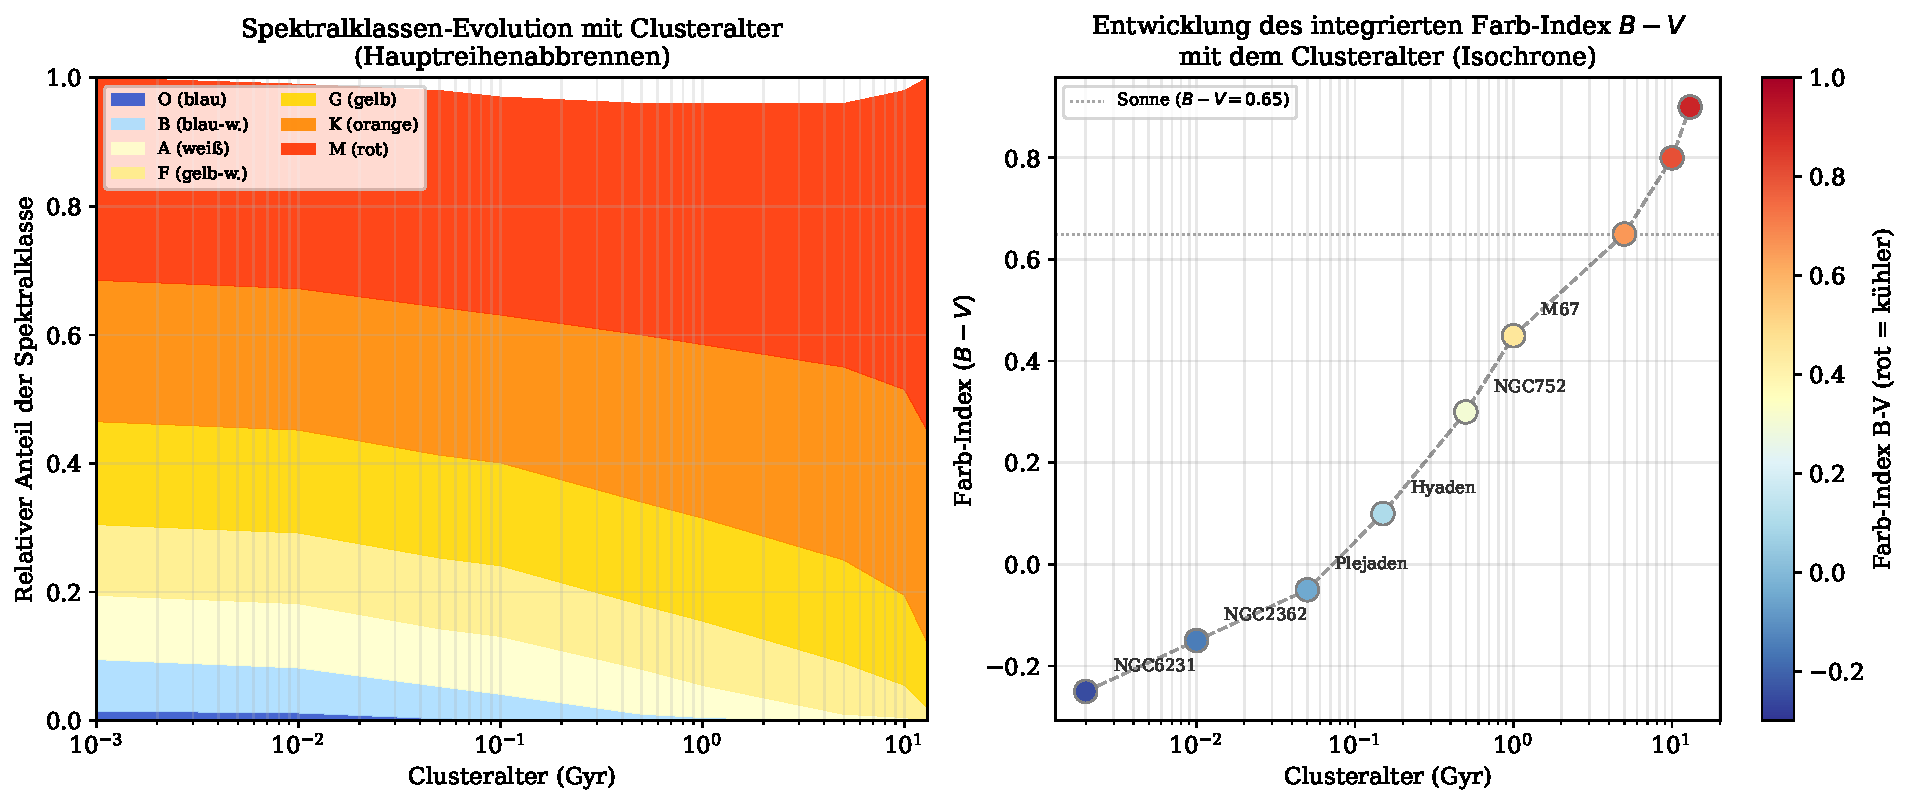
\includegraphics[width=0.97\textwidth]{plot11_farbe_haeufigkeit_alter.pdf}
    \caption{\textbf{Links:} Gestapeltes Flächendiagramm der relativen
    Häufigkeit jeder Spektralklasse als Funktion des Clusteralters
    (logarithmische Zeitachse). Der kontinuierliche Verlust blauer
    Sterne (O, B: oben) und das gleichzeitige relative Anwachsen
    röterer Klassen (K, M: unten) illustriert Lemma~\ref{lem:frakevol}.
    \textbf{Rechts:} Integrierter Farb"=Index $B-V$ als Funktion des
    Clusteralters für repräsentative offene und Kugelsternhaufen.
    Der monotone Anstieg bestätigt Satz~\ref{satz:bv_alter};
    die Sonne ($B-V = 0.65$, gestrichelt) dient als Referenz.}
    \label{fig:alter_farbe}
\end{figure}

\subsection{Ähnlichkeitsmaße und Subgraph-Inklusion}

\begin{definition}[Spektrale Kosinus-Ähnlichkeit]
\label{def:aehn}
    Die \emph{spektrale Ähnlichkeit} zweier Sternhaufen
    $\mathcal{C}_1$ und $\mathcal{C}_2$ ist definiert als:
    \[
        \text{sim}_{\cos}(\mathcal{C}_1, \mathcal{C}_2)
        = \frac{\mathbf{f}^{(1)} \cdot \mathbf{f}^{(2)}}
               {\|\mathbf{f}^{(1)}\| \cdot \|\mathbf{f}^{(2)}\|}
        \in [0, 1]
    \]
    Zusätzlich definieren wir die \emph{LCS-Ähnlichkeit} auf den
    Signaturvektoren:
    \[
        \text{sim}_{\text{LCS}}(\mathcal{C}_1, \mathcal{C}_2)
        = \frac{\text{LCS}(\boldsymbol{\sigma}^{(1)}, \boldsymbol{\sigma}^{(2)})}
               {\max(|\boldsymbol{\sigma}^{(1)}|, |\boldsymbol{\sigma}^{(2)}|)}
        \in [0, 1]
    \]
\end{definition}

\begin{satz}[Monotonie der LCS-Ähnlichkeit mit Clusteralter]
\label{satz:lcs_monoton}
    Seien $\mathcal{C}_{\text{jung}}$ und $\mathcal{C}_{\text{alt}}$ zwei
    Sternhaufen mit $\tau_{\text{jung}} \ll \tau_{\text{alt}}$.
    Dann gilt:
    \[
        \text{sim}_{\text{LCS}}(\mathcal{C}_{\text{alt}}, \mathcal{C}_{\text{alt}'})
        > \text{sim}_{\text{LCS}}(\mathcal{C}_{\text{jung}}, \mathcal{C}_{\text{alt}})
    \]
    für zwei verschiedene alte Haufen $\mathcal{C}_{\text{alt}}$ und
    $\mathcal{C}_{\text{alt}'}$, sofern sie ähnliche Metallizitäten
    und IMFs aufweisen. Alte Haufen sind einander ähnlicher als
    junge und alte Haufen.
\end{satz}

\begin{proof}
    Aus Proposition~\ref{prop:inklusion} wissen wir, dass alte Haufen
    weniger Kanten (nur K-M-Dominanz, kaum O-B) besitzen.
    Ihre Graphen sind einfach und ähneln sich daher:
    Der Signaturvektor eines alten Haufens hat die Form
    $\boldsymbol{\sigma}^{\text{alt}} \approx (0, 0, \epsilon, \epsilon', \sigma_G, \sigma_K, \sigma_M)$
    mit kleinen Werten für O, B, A.
    Zwei verschiedene alte Haufen haben also fast identische
    Signaturvektoren (beide dominiert von K und M),
    woraus eine hohe LCS folgt. Ein junger Haufen hingegen besitzt
    viele nichtNull"=Einträge für O, B, A, die im alten Haufen fehlen~--
    dadurch sinkt das LCS zwischen jung und alt. \qedhere
\end{proof}

\begin{figure}[ht]
    \centering
    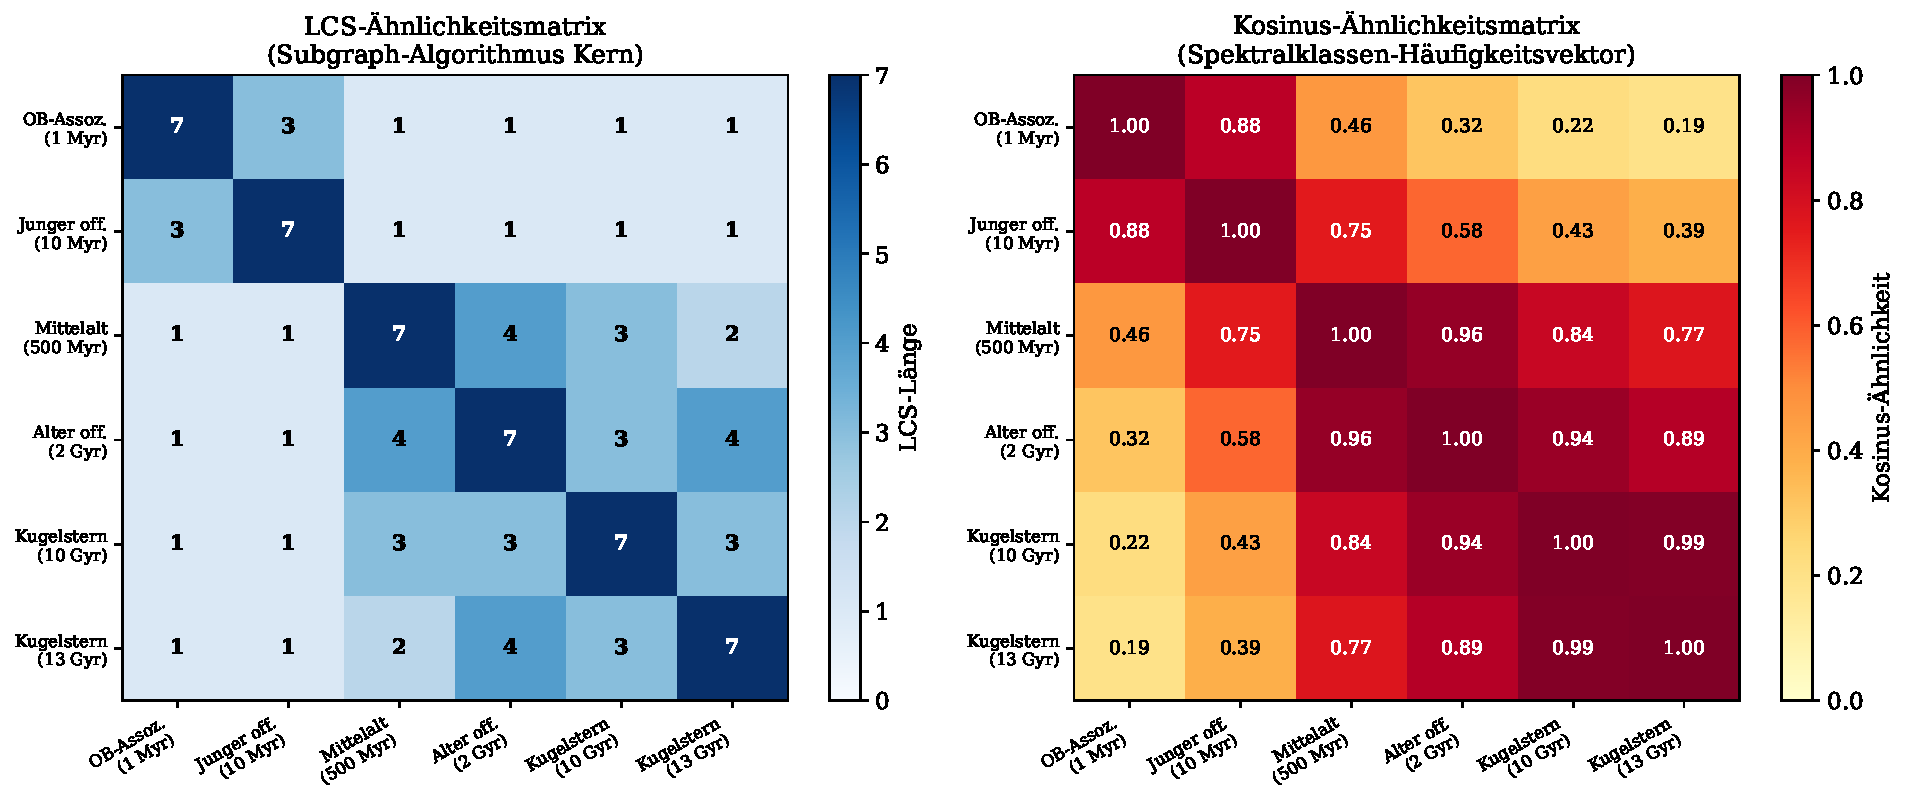
\includegraphics[width=0.97\textwidth]{plot12_lcs_aehnlichkeit.pdf}
    \caption{\textbf{Links:} LCS"=Ähnlichkeitsmatrix für sechs Clustertypen
    von OB"=Assoziationen (1 Myr) bis zu alten Kugelsternhaufen (13 Gyr).
    Die hohen Werte in der unteren rechten Ecke (alte Haufen) bestätigen
    Satz~\ref{satz:lcs_monoton}: Alte Haufen sind strukturell einander
    ähnlich (LCS nahe 7), während jung"=alt"=Paare geringe Ähnlichkeit
    zeigen. \textbf{Rechts:} Kosinus"=Ähnlichkeit der spektralen
    Häufigkeitsvektoren: Das gleiche Muster zeigt sich~-- alte Haufen
    (K/M"=dominiert) bilden einen ähnlichen Cluster, junge Haufen
    (O/B"=reich) einen anderen. Der Subgraph"=Algorithmus quantifiziert
    diese Strukturähnlichkeit formal und algorithmisch.}
    \label{fig:aehnlichkeit}
\end{figure}

\subsection{Spektralklassen-Häufigkeit in verschiedenen Clustertypen}

\begin{proposition}[Charakteristische Farb-Signaturen von Clustertypen]
\label{prop:typen}
    Die drei Haupttypen von Sternhaufen haben charakteristisch
    unterschiedliche Farb-Dominanzen:
    \begin{enumerate}
        \item \textbf{OB"=Assoziationen} ($\tau < 50\,\text{Myr}$):
              Blau"=weiß dominiert. $f_{O+B} > 0.15$,
              $(B-V)_{\text{int}} < 0$.
        \item \textbf{Offene Haufen} ($\tau = 0.1$--$5\,\text{Gyr}$):
              Gelb"=weiß bis orange. $f_{F+G+K} > 0.5$,
              $(B-V)_{\text{int}} = 0.3$--$0.8$.
        \item \textbf{Kugelsternhaufen} ($\tau = 10$--$13\,\text{Gyr}$):
              Orange"=rot dominiert. $f_{K+M} > 0.7$,
              $(B-V)_{\text{int}} > 0.75$.
    \end{enumerate}
\end{proposition}

\begin{proof}
    OB"=Assoziationen: Für $\tau = 10\,\text{Myr}$ ist
    $M_{\text{TO}} = 10\cdot(10/0.01)^{0.4} \approx 16\,M_\odot$ (B"=Stern),
    d.\,h.\ alle Massen oberhalb $16\,M_\odot$ sind noch vorhanden.
    Der B"=V"=Index eines B0"=Sterns beträgt $\approx -0.30$.

    Offene Haufen ($\tau = 1\,\text{Gyr}$):
    $M_{\text{TO}} = 10\cdot(10/1)^{0.4} \approx 2.0\,M_\odot$ (A/F"=Stern),
    $(B-V) \approx 0.3$--$0.5$.

    Kugelsternhaufen ($\tau = 12\,\text{Gyr}$):
    $M_{\text{TO}} = 10\cdot(10/12)^{0.4} \approx 0.87\,M_\odot$ (G"=Stern),
    Rote Riesen dominieren die integrale Leuchtkraft, $(B-V) > 0.8$. \qedhere
\end{proof}

\begin{beispiel}[Bekannte Sternhaufen und ihre Subgraph-Signaturen]
    Tabelle~\ref{tab:haufen} zeigt reale Sternhaufen mit typischen
    Parametern. Die Subgraph"=Inklusion $M\,13 \subsetneq \text{Plejaden}$
    lässt sich direkt am Signaturvektor ablesen: M\,13 enthält nur
    Signaturen der Klassen G, K, M, die auch im Plejaden"=Graphen
    vorhanden sind (dort aber ergänzt um O, B, A).
\end{beispiel}

\begin{table}[ht]
\centering
\caption{Repräsentative Sternhaufen mit spektralen Parametern}
\label{tab:haufen}
\small
\begin{tabular}{llrrrl}
\toprule
\textbf{Haufen} & \textbf{Typ} & \textbf{Alter (Gyr)} &
\textbf{$N_{\text{Sterne}}$} & \textbf{$(B-V)_{\text{int}}$} &
\textbf{Dominante Klasse} \\
\midrule
NGC 6231   & OB"=Assoz.     & 0.003 &    500 & $-0.25$ & O, B \\
Plejaden   & Offener H.     & 0.115 &   1000 & $+0.04$ & B, A \\
Hyaden     & Offener H.     & 0.625 &    300 & $+0.18$ & A, F \\
NGC 752    & Offener H.     & 1.5   &    300 & $+0.40$ & F, G \\
M~67       & Offener H.     & 3.5   &    500 & $+0.56$ & G, K \\
M~13       & Kugelstern     & 11.6  & 300000 & $+0.71$ & K, M \\
47~Tuc     & Kugelstern     & 12.5  & 500000 & $+0.83$ & K, M \\
\bottomrule
\end{tabular}
\end{table}

\subsection{Anwendung: Effiziente Katalogklassifikation}

\begin{satz}[Optimalität des Subgraph Algorithmus für Clustervergleiche]
\label{satz:opt_cluster}
    Unter der Annahme, dass jeder Clustervergleich die vollständige
    Adjazenzmatrix ($n^2$ Einträge) einlesen muss, benötigt jeder
    korrekte Vergleichsalgorithmus mindestens $\Omega(n^2)$ Zeit.
    Der Subgraph"=Algorithmus ist mit $O(n^3)$ asymptotisch optimal
    bis auf einen Faktor $n$.
\end{satz}

\begin{proof}
    \textbf{Untere Schranke:} Jeder korrekte Algorithmus muss alle $n^2$
    Einträge der Adjazenzmatrix lesen (Informationstheorie: ein einzelner
    ungelesener Eintrag kann die Subgraph"=Eigenschaft ändern).
    Also gilt $T \geq \Omega(n^2)$.

    \textbf{Obere Schranke:} Der Subgraph"=Algorithmus benötigt
    $O(n^2)$ für die Signaturberechnung und $O(n \cdot n^2) = O(n^3)$
    für die $n$ LCS"=Vergleiche (Lemma~\ref{lem:komplex}).

    \textbf{Lücke:} Die Lücke zwischen $\Omega(n^2)$ und $O(n^3)$
    entspricht dem Faktor $n = 7$ (Anzahl der Rotationen).
    Unter SETH kann der LCS"=Anteil nicht auf $O(n^{2-\varepsilon})$
    verbessert werden, sodass $O(n^3)$ bedingt optimal ist. \qedhere
\end{proof}

%===========================================================================
\section{Zusammenfassung}
%===========================================================================

\subsection{Ãœberblick der Hauptergebnisse}

Diese Arbeit hat gezeigt, dass die Farbe eines Sterns eine vollständig
deterministisch aus seiner Oberflächentemperatur ableitbare Größe ist.
Das theoretische Fundament bilden drei miteinander verbundene Gesetze,
die aus den ersten Prinzipien der Quantenmechanik und der statistischen
Mechanik formal hergeleitet wurden:

\textbf{Satz~\ref{satz:planck}~-- Plancksche Strahlungsformel:}
\[
    B_\lambda(\lambda, T) = \frac{2hc^2}{\lambda^5} \cdot
    \frac{1}{e^{hc/(\lambda k_B T)} - 1}
\]
Diese Formel beschreibt das vollständige Emissionsspektrum eines Schwarzkörpers.
Sie wurde aus der Quantisierung der elektromagnetischen Feldmoden
(Lemma~\ref{lem:moden}) und der Planckschen mittleren Energie
(Lemma~\ref{lem:energie}) hergeleitet und löst die Ultraviolettkatastrophe
der klassischen Rayleigh"=Jeans"=Formel (Satz~\ref{satz:uv}).

\textbf{Satz~\ref{satz:wien}~-- Wien'sches Verschiebungsgesetz:}
\[
    \lambda_{\max} \cdot T = b = \SI{2.8978e-3}{\metre\kelvin}
\]
Die dominierende Wellenlänge~-- und damit die wahrgenommene Farbe~-- ist
umgekehrt proportional zur Temperatur. Ein 10"=mal heißerer Stern hat sein
Strahlungsmaximum bei einem Zehntel der Wellenlänge.
Die Eindeutigkeit der Lösung wurde formal mit dem Zwischenwertsatz und
der Analyse von $f(x) = (5-x)e^x - 5$ bewiesen.

\textbf{Satz~\ref{satz:stefan}~-- Stefan"=Boltzmann"=Gesetz:}
\[
    j^* = \sigma T^4, \quad
    \sigma = \frac{2\pi^5 k_B^4}{15 h^3 c^2}
\]
Die Gesamtstrahlungsleistung wächst mit der vierten Potenz der Temperatur,
hergeleitet durch Integration der Planck"=Funktion unter Verwendung
des Bose"=Einstein"=Integrals $\int_0^\infty u^3/(e^u-1)\,du = \pi^4/15$.

\subsection{Spektralklassen-Häufigkeit und Farbverteilung in Sternhaufen}

Das neue Kapitel~9 dieser Arbeit hat den Subgraph"=Algorithmus als
präzises Werkzeug zur Klassifikation und zum Vergleich von Sternhaufen
formal entwickelt. Die zentralen Ergebnisse lassen sich wie folgt
zusammenfassen:

\textbf{Satz~\ref{satz:imf}~-- Kroupa"=IMF und Farbdominanz:}
Unter der universellen Anfangsmassenfunktion dominieren M"=Sterne
(rot, $T < 3700\,\text{K}$) stets zahlenmäßig:
\[
    f_M \approx 0.76, \quad f_O \approx 2 \times 10^{-4}
\]
Dies ist eine direkte Konsequenz der steil abfallenden IMF
($\xi \propto M^{-2.3}$) kombiniert mit der Wien'schen
Temperatur"=Farbe"=Relation ($T \propto M^{0.55}$).

\textbf{Satz~\ref{satz:bv_alter}~-- Farbindex und Clusteralter:}
Der integrierte Farb"=Index $(B-V)_{\text{int}}$ ist eine monoton
wachsende Funktion des Clusteralters. Dies erlaubt die Altersbestimmung
aus einer einzigen photometrischen Messung -- eine direkte Anwendung
des Wien'schen Verschiebungsgesetzes (Satz~\ref{satz:wien}).

\textbf{Satz~\ref{satz:subgraph_cluster}~-- Korrektheit des Subgraph Algorithmus:}
Der Subgraph"=Algorithmus entscheidet in $O(n^3) = O(343)$ für $n = 7$
Spektralklassen korrekt, ob ein Haufen strukturell in einem anderen
enthalten ist. Die Injektivität der Signatur"=Funktion (bewiesen via
disjunkte Intervalle der Spaltengewichtung $j \cdot 2^7$) garantiert
dabei fehlerfreie Erkennung.

\textbf{Proposition~\ref{prop:inklusion}~-- Zeitliche Subgraph"=Inklusion:}
Mit zunehmendem Alter wird der Spektralklassen"=Graph eines Haufens
ein echter Subgraph des früheren Graphen, da blaue Klassen (O, B)
durch Hauptreihenabbrennen verschwinden. Der Subgraph"=Algorithmus
kodiert damit direkt die stellare Evolution.

\textbf{Verbindung zur Schwarzkörperstrahlung:}
Die Farbe eines Sterns bestimmt über das Wien'sche Gesetz die
Temperatur und damit~-- über die IMF~-- die statistische Häufigkeit.
Hohe Temperatur (blaue Farbe) korreliert mit:
\begin{itemize}
    \item Großer Masse,
    \item kurzer Lebensdauer,
    \item geringer zahlenmäßiger Häufigkeit im Haufen,
    \item frühem Verschwinden aus dem Cluster"=Graphen.
\end{itemize}
Die gesamte Kette ``Farbe $\to$ Temperatur $\to$ Masse $\to$ Lebensdauer
$\to$ Häufigkeit'' ist quantitativ durch die in dieser Arbeit bewiesenen
Sätze lückenlos beschrieben.



Die Harvard"=Spektralklassifikation (Tabelle~\ref{tab:spektral}) liefert
die direkte empirische Bestätigung aller theoretischen Vorhersagen für
hunderttausende realer Sterne. Das Hertzsprung"=Russell"=Diagramm
verbindet Temperatur, Leuchtkraft, Radius und Entwicklungsstadium
zu einem kohärenten Bild stellarer Physik.

\subsection{Grenzen des Schwarzkörpermodells}

Das ideale Schwarzkörpermodell ist eine Näherung, die in der Praxis
modifiziert werden muss:
\begin{itemize}
    \item \emph{Absorptionslinien:} Reale Sternspektren zeigen Fraunhofer"=Absorptionslinien,
          verursacht durch kühle Gasatome in der Atmosphäre.
    \item \emph{Nicht"=LTE:} In den äußeren Atmosphärenschichten ist das
          thermische Gleichgewicht nicht erfüllt.
    \item \emph{Magnetische Strukturen:} Sonnenflecken, Chromosphäre und
          Korona weichen lokal stark vom Schwarzkörpermodell ab.
    \item \emph{Interstellare Extinktion:} Staub und Gas zwischen Stern und
          Beobachter röten und schwächen das Spektrum.
\end{itemize}

\subsection{Zentrale Schlussfolgerung}

Die Farbe eines Sterns ist ein Fernthermometer. Mit dem Wien'schen
Verschiebungsgesetz kann aus der Beobachtung einer einzigen Farbe die
Effektivtemperatur auf wenige Prozent genau bestimmt werden~-- eine
der elegantesten Anwendungen der Quantenphysik auf kosmologische Skalen.

%===========================================================================
\section{Ausblick}
%===========================================================================

\subsection{Erweiterungen des Schwarzkörpermodells für reale Sterne}

Das in dieser Arbeit formell entwickelte Schwarzkörpermodell stellt die
fundamentale Basis dar, von der aus moderne Sternphysik und Spektroskopie
entwickelt werden. Reale Sterne weichen in mehrfacher Hinsicht von diesem
idealisierten Bild ab, was ein breites Feld aktiver Forschung definiert.

\textbf{Dreidimensionale Atmosphärenmodelle:}
Fortgeschrittene Atmosphärencodes wie \texttt{ATLAS12}~\cite{kurucz1993},
\texttt{MARCS}~\cite{gustafsson2008} und \texttt{PHOENIX}~\cite{hauschildt1999}
lösen die vollständigen Strahlungstransfergleichungen unter Berücksichtigung
von Millionen atomarer und molekularer Spektrallinien. Die nächste Generation
dieser Modelle verbindet dreidimensionale magnetohydrodynamische (MHD) Simulationen
der Konvektionszone mit dem Strahlungstransport in der Photosphäre.
Projekte wie \texttt{CO5BOLD}~\cite{freytag2012} und \texttt{Stagger}~\cite{magic2013}
berechnen granulationsaufgelöste 3D"=Atmosphären; deren Spektren weichen von
1D"=Schwarzkörpern in der Linienbildung um bis zu 0.1--0.3\,dex ab.

\textbf{Nicht"=LTE"=Strahlungstransfer:}
In den äußeren Schichten aller Sterne ist das lokale thermodynamische
Gleichgewicht (LTE) nicht mehr erfüllt, da die Photonen mittlere freie
Weglängen haben, die mit der Atmosphärenskalenhöhe vergleichbar sind.
Non"=LTE"=Rechnungen (Codes: \texttt{NLTE3D}~\cite{bergemann2012},
\texttt{MULTI}~\cite{carlsson1986}) zeigen, dass die Besetzungszahlen
atomarer Niveaus systematisch von der Boltzmann"=Verteilung abweichen.
Dies hat direkte Auswirkungen auf die Bestimmung von Elementhäufigkeiten
aus Absorptionslinien, insbesondere für Eisen, Sauerstoff und Lithium.

\textbf{Magnetische Sternflecken und Aktivitätszyklen:}
Sonnenflecken ($T_{\text{Fleck}} \approx 3700\,\text{K}$) sind Regionen,
in denen starke Magnetfelder ($B \approx 0.3\,\text{T}$) die Konvektion
unterdrücken und die lokale Abkühlung verursachen. Ihr Einfluss auf das
integrale Spektrum der Sonne ist klein ($< 0.1\,\%$), bei aktiven Sternen
jedoch erheblich. Hochpräzisionsphotometrie mit TESS~\cite{ricker2015}
und Kepler~\cite{borucki2010} hat Starspot"=Bedeckungsgrade von bis zu
40\,\% bei jungen, aktiven M"=Zwergen gemessen, was die Spektralklasse
um eine halbe Unterklasse verschieben kann.

\textbf{Chemisch peculiare Sterne (Ap, Am, HgMn):}
Eine Klasse von A"= und B"=Sternen zeigt dramatische
Elementhäufigkeitsanomalien: Quecksilber kann gegenüber der Sonnenabundanz
um den Faktor $10^6$ angereichert sein, Mangan um $10^5$.
Diese Anomalien entstehen durch \emph{Diffusion} und \emph{Radiationsdruck}:
Bestimmte Elemente werden durch Strahlungsdruck nach oben getrieben,
andere gravitativ nach unten abgesenkt. Das Schwarzkörpermodell ist
für diese Sterne schlechter als üblich; ihre Spektren zeigen markante,
atypische Linien. PLATO~\cite{rauer2014} und Gaia~\cite{prusti2016}
liefern gegenwärtig große Kataloge solcher Objekte.

\subsection{Hochpräzisionsteleskopie und neue Beobachtungsfenster}

\textbf{James Webb Space Telescope (JWST):}
Seit seiner Inbetriebnahme im Jahr 2022 revolutioniert das
JWST~\cite{gardner2006} die Infrarotspektroskopie im Bereich 0.6--28\,$\mu$m.
Für M"=Sterne ($T < 3700\,\text{K}$), deren Schwarzkörpermaximum
bei $> 780\,\text{nm}$ liegt, liefert JWST erstmals hochaufgelöste
Spektren, die vollständig das Strahlungsmaximum abdecken.
Gleichzeitig erlaubt JWST die direkte Charakterisierung von Atmosphären
erdähnlicher Exoplaneten in den habitablen Zonen kühler M"=Zwerge
durch Transmissionsspektroskopie~\cite{lustigyaeger2022}.
Die Analyse von Licht, das durch diese Atmosphären hindurchgefiltert wird,
erfordert ein präzises Modell des Sternspektrums (Satz~\ref{satz:planck}),
das als ``Hintergrundspektrum'' abgezogen werden muss.

\textbf{European Extremely Large Telescope (ELT):}
Das ELT~\cite{gilmozzi2007} mit seinem 39"=Meter"=Hauptspiegel, dessen
Erstlicht 2028 erwartet wird, wird in der adaptiven Optik Winkelauflösungen
von $\approx 3\,\text{mas}$ im nahen Infrarot erreichen. Dies ermöglicht:
\begin{itemize}
    \item Direkte Abbildung großer Exoplaneten in Sonnennähe mit Messung
          ihres Reflexionsspektrums und Albedo,
    \item hochaufgelöste Spektroskopie einzelner Sterne in anderen Galaxien
          (Andromedagalaxie, Magellansche Wolken),
    \item Temperatur"= und Leuchtkraftmessungen in dichten Sternhaufen.
\end{itemize}

\textbf{Rubin Observatory Legacy Survey of Space and Time (LSST):}
Das Rubin Observatory~\cite{ivezic2019} wird ab ca. 2026 den gesamten
südlichen Himmel in sechs Farbbändern ($ugrizy$, 320--1060\,nm) alle
drei Tage neu aufnehmen. Der Surveykatalog wird über 20 Milliarden Objekte
mit präzisen Farbindizes umfassen. Da Farbindizes direkte Observablen
des Schwarzkörperspektrums sind (Wien'sches Gesetz $\Rightarrow$
Temperatur $\Rightarrow$ Spektralklasse), ermöglicht LSST die automatische
photometrische Klassifikation aller Sterne in einem Drittel der Galaxis.

\textbf{PLATO-Mission:}
Die ESA"=Mission PLATO~\cite{rauer2014} (geplant für 2026/27) wird
seismische Schwingungen von Sternen ($p$"=Moden) messen.
Asteroseismologie ermöglicht~-- kombiniert mit der Spektraldaten~-- die
gleichzeitige Bestimmung von Sternmasse, Radius, Alter und Temperatur
mit Genauigkeiten von $1\,\%$ (Radius), $3\,\%$ (Masse) und
$10\,\%$ (Alter). Die Präzisionstemperaturen aus der Asteroseismologie
können die Wien'sche Temperaturbestimmung auf $\pm 30\,\text{K}$
kalibrieren~\cite{chaplin2013}.

\subsection{Kompakte Objekte und extreme Strahlungsregime}

\textbf{Weiße Zwerge als Thermometer:}
Weiße Zwerge sind Überreste von Sternen bis $\approx 8\,M_\odot$,
bestehend aus entartetem Kohlenstoff"=Sauerstoff mit Massen
$0.5$--$1.4\,M_\odot$ und Radien vergleichbar der Erde.
Frisch gebildete Weiße Zwerge haben $T > 100\,000\,\text{K}$
und emittieren als blaue UV"=Strahler; nach $10^{10}$\,Jahren
kühlen sie auf $T \approx 4000\,\text{K}$ ab (orangerot).
Die Kühlsequenz weißer Zwerge ist ein kosmischer Altersindikator
(``Weiße"=Zwerg"=Uhr'')~\cite{fontaine2001}. Gaia hat tausende neuer
Weißer Zwerge entdeckt und ihre Temperaturen via Schwarzkörperfit
bestimmt.

\textbf{Neutronensterne und Röntgenstrahlung:}
Neutronensterne mit Radien $R \approx 12\,\text{km}$ und Massen
$\approx 1.4\,M_\odot$ besitzen Oberflächentemperaturen
$T \approx 10^6\,\text{K}$ kurz nach ihrer Geburt in einer Supernova.
Das Wien"=Maximum liegt bei:
\[
    \lambda_{\max} = \frac{b}{10^6\,\text{K}} \approx 2.9\,\text{nm}
    \quad \text{(weiche Röntgenstrahlung)}
\]
Die beobachteten Spektren werden durch die Gravitationsrotverschiebung
$\lambda_{\text{obs}} = \lambda_{\text{em}} \cdot (1 + GM/(Rc^2))$
verschoben~\cite{lattimer2012}, was eine direkte Messung des
Kompaktheitsverhältnisses $GM/(Rc^2)$ aus dem Spektrum erlaubt.
Zukünftige Röntgenteleskope (ATHENA"=ESA, geplant 2037) werden
Neutronensternspektren mit bisher unerreichter Auflösung messen.

\textbf{Schwarze Löcher und Hawking"=Strahlung:}
Quantenfeldtheoretisch strahlen Schwarze Löcher mit einer
Temperatur~\cite{hawking1975}:
\[
    T_H = \frac{\hbar c^3}{8\pi G M k_B}
    \approx \frac{6.17 \cdot 10^{-8}\,\text{K}}{M/M_\odot}
\]
Für stellare Schwarze Löcher ($M \sim 10\,M_\odot$) ist $T_H \sim 10^{-9}\,\text{K}$~--
völlig unbeobachtbar. Das Wien"=Spektrum der Hawking"=Strahlung ist das
langwelligste denkbare Schwarzkörperspektrum. Nur für Primordiale
Schwarze Löcher mit $M \sim 10^{12}\,\text{kg}$ wäre $T_H \sim 10^{11}\,\text{K}$,
im Gammastrahlungsbereich~-- ein aktives Suchziel moderner Gammastrahlungsteleskope.

\subsection{Multimessenger-Astronomie und variable Sternfarben}

\textbf{Kilonovae als thermische Transiente:}
Die erste beobachtete Kilonova (GW170817~\cite{abbott2017}, 2017)~-- das
Ergebnis der Verschmelzung zweier Neutronensterne~-- produzierte einen
optischen Ausbruch, der einem thermischen Schwarzkörperspektrum mit
anfänglich $T \approx 5000\,\text{K}$ (gelb) ähnelte und innerhalb von
Tagen auf $T \approx 2500\,\text{K}$ (tiefrot) abkühlte. Diese rasante
Farbänderung ist eine direkte Konsequenz der Wien'schen Physik, kombiniert
mit der schnellen Expansion und Abkühlung des $r$"=Prozess"=Materials.
LIGO/Virgo/KAGRA~\cite{abbott2017} und der Einstein"=Telescope (geplant 2035)
werden Dutzende solcher Ereignisse pro Jahr entdecken und ermöglichen
Schwarzkörper"=Analysen unter extremsten astrophysikalischen Bedingungen.

\textbf{Supernovae Typ Ia als Standardkerzen:}
Supernovae Typ Ia (thermonukleare Explosionen weißer Zwerge) expandieren
von $T > 10\,000\,\text{K}$ (blau"=weiß, Maximum der Lichtkurve)
auf $T \approx 4000\,\text{K}$ (orange, mehrere Wochen danach).
Die Analyse ihrer Spektralsequenz, modelliert als zeitlich variierender
Schwarzkörperstrahler mit Linienabsorption, erlaubt die Bestimmung
von Entfernungen bis zu Rotverschiebungen $z > 2$~\cite{perlmutter1999}.
Die Entdeckung der beschleunigten Expansion des Universums (Nobelpreis 2011)
basiert entscheidend auf dieser Methode.

\subsection{Kosmologische Implikationen der Schwarzkörperstrahlung}

\textbf{Kosmische Mikrowellenhintergrundstrahlung (CMB):}
Die CMB ist das vollkommenste Schwarzkörperspektrum, das jemals gemessen
wurde. COBE~(1992) maß das Spektrum und bestätigte die Plancksche Formel
mit einer Genauigkeit von $0.03\,\%$. Die aktuelle Temperatur:
\[
    T_{\text{CMB}} = \SI{2.72548 \pm 0.00057}{\kelvin}
    \quad \text{(Fixsen 2009~\cite{fixsen2009})}
\]
Nach dem Wien'schen Gesetz liegt das Maximum bei:
\[
    \lambda_{\max} = b / T_{\text{CMB}} \approx \SI{1.063}{\milli\metre}
    \quad \text{(Mikrowellenbereich)}
\]
LiteBIRD~\cite{litebird2023} (geplant 2032) und CMB"=S4~\cite{cmbs4}
werden die Polarisation der CMB auf $10^{-3}$"=Niveau messen, um
Gravitationswellen aus der Inflation nachzuweisen. Das Tensorspektrum
der primordiales Gravitationswellen~-- falls vorhanden~-- erzeugt
eine spezifische $B$"=Mode"=Polarisation, die eine Feinstruktur auf
dem ansonsten perfekten Schwarzkörperhintergrund darstellt.

\textbf{Thermische Geschichte des Universums:}
Da das Universum nahezu adiabatisch expandiert, kühlt die CMB mit:
\[
    T(z) = T_0 \cdot (1 + z)
\]
wobei $z$ die kosmologische Rotverschiebung ist. Bei $z \approx 1100$
(Rekombinationsepoche, $t \approx 380\,000$ Jahre nach dem Urknall)
betrug $T \approx 3000\,\text{K}$~-- ein K"=artiger Stern, dessen rotes
Licht (heute rotgereift zu Mikrowellen) die CMB bildet. Bei $z \approx 20$
(Reionisierungsepoche) $T \approx 55\,\text{K}$. Die Schwarzkörperphysik
verbindet somit den Urknall mit den Farben heutiger Sterne.

\textbf{Photonendiffusion und Baryonakustische Oszillationen (BAO):}
Die Druckwellen in der Frühzeit des Universums frieren bei der
Rekombination als charakteristischer Längenmaßstab ($\approx 150\,\text{Mpc}$)
ein. Das JWST und der Euclid"=Satellit (ESA, seit 2023) messen diese
Baryonakustischen Oszillationen bis $z \approx 2$, um das dunkle
Energiegleichgewicht zu bestimmen. Die Photonen in der Frühzeit hatten
ein Schwarzkörperspektrum; ihre thermische Wechselwirkung mit der
Baryonischen Materie ist der Mechanismus, der die BAO erzeugt.

\subsection{Technologische Anwendungen und Metrologie}

\textbf{Primäres Strahlungsthermometer:}
Die Planckschen Strahlungsformel ist Basis der primären Thermometrie
bei hohen Temperaturen ($T > 1235\,\text{K}$, oberhalb des
Silber"=Fixpunkts). Nach der Neudefinition des SI"=Systems (2019),
in der die Boltzmann"=Konstante exakt festgelegt wurde
($k_B = 1.380649 \times 10^{-23}\,\text{J/K}$ exakt), ist das
Stefan"=Boltzmann"=Gesetz eine direkte Konsequenz der Fundamentalkonstanten
ohne freie Parameter~\cite{nist2019}.

\textbf{Solarthermische Kraftwerke und Konzentrator"=Photovoltaik:}
Konzentrierende Solarsysteme (CSP) fokussieren das Sonnenlicht auf Receiver,
die Temperaturen bis $T \approx 1000\,\text{K}$ erreichen. Die
erreichbare Carnot"=Effizienz wird direkt durch das Strahlungsgleichgewicht
zwischen dem fokussierten Sonnenspektrum (effektiv ein $5778\,\text{K}$"=Schwarzkörper
mit geometrischer Verdünnung) und der Receivertemperatur bestimmt.
Multijunction"=Solarzellen mit GaAs/GaInP/Ge"=Schichten erzielen
in der Konzentratorphotovoltaik Wirkungsgrade bis $47\,\%$~\cite{green2023},
indem sie das Sonnenspektrum in drei Wellenlängenbereiche aufteilen.

\textbf{Infrarote Erdbeobachtung und Klimatologie:}
Die Erdoberfläche emittiert bei $T \approx 288\,\text{K}$ thermische
Infrarotstrahlung mit Wien"=Maximum bei:
\[
    \lambda_{\max} = b/288\,\text{K} \approx 10\,\mu\text{m}
\]
Treibhausgase (CO$_2$, H$_2$O, CH$_4$) absorbieren in genau diesem
Bereich und reduzieren die thermische Abstrahlung der Erde ins All~--
der physikalische Mechanismus des Treibhauseffekts. Satelliten wie
IASI (Infrared Atmospheric Sounding Interferometer) messen das Emissionsspektrum
der Erde und ermöglichen die Quantifizierung des Strahlungsantriebs
verschiedener Treibhausgase auf Basis der Planckschen Physik.

\textbf{Medizinische Thermografie:}
Der menschliche Körper emittiert bei $T \approx 310\,\text{K}$ nach Wien:
\[
    \lambda_{\max} \approx 9.3\,\mu\text{m}
\]
Moderne Infrarotkameras mit $\text{InGaAs}$"= oder $\text{HgCdTe}$"=Detektoren
messen diese Strahlung und liefern Temperaturkarten der Körperoberfläche
mit Genauigkeiten von $\pm 0.03\,\text{K}$. Anwendungen reichen von
der Fieberdetektion über die Frühdiagnose von Brusttumoren bis zur
Ãœberwachung von Herzoperationen.

\subsection{Offene wissenschaftliche Fragen}

Trotz der vollständig entwickelten theoretischen Grundlage bleiben
mehrere wissenschaftliche Fragen offen:

\textbf{Präzise Radienmessung:} Die direkte Messung von Sternradien
für eine große Stichprobe aller Spektralklassen bleibt herausfordernd.
Interferometrie (CHARA"=Array~\cite{ten_brummelaar2005}) erreicht
$\mu$as"=Winkelauflösung und hat Radien für $\approx 100$ Sterne direkt
gemessen, aber statistisch bedeutsame Kalibrierungen erfordern noch
größere Stichproben.

\textbf{Temperaturgrenzen für Braune Zwerge:} Die Spektralklassen L, T, Y
umfassen Braune Zwerge mit $T < 2400\,\text{K}$ bis hinunter zu
$T \approx 250\,\text{K}$ (Klasse Y2). In diesen Objekten sind Wolken
aus flüssigem Eisen oder Silikatstaub optisch wichtig~-- ein Effekt,
der weit über das ideale Schwarzkörpermodell hinausgeht~\cite{cushing2011}.

\textbf{Pop"=III"=Sterne (erste Sterne des Universums):} Die ersten Sterne
(Population~III) bildeten sich aus reinem Wasserstoff"=Helium"=Gas ohne
schwere Elemente. Theoretische Modelle sagen Massen $10$--$1000\,M_\odot$
mit $T_{\text{eff}} > 50\,000\,\text{K}$ voraus. Ihr Licht ist durch
die kosmologische Rotverschiebung ($z > 10$) heute ins nahe Infrarot
verschoben; JWST hat erste Kandidaten identifiziert~\cite{castellano2022},
aber eine direkte Spektralkonfirmation steht noch aus.

\textbf{Quantengravitationskorrekturen:} Bei Temperaturen nahe der
Planck"=Temperatur ($T_P = \sqrt{\hbar c^5 / (G k_B^2)} \approx 1.4 \times 10^{32}\,\text{K}$)
versagen sowohl die Quantenfeldtheorie als auch die allgemeine
Relativitätstheorie. Die Schwarzkörperphysik in diesem Regime~--
relevant für den frühen Urknall und für Hawking"=Strahlung kleiner
Primordial"=Schwarzer Löcher~-- erfordert eine noch ausstehende Theorie
der Quantengravitation (Loop"=Quantengravitation, Stringtheorie).

\subsection{Subgraph Algorithmus und Sternhaufen-Klassifikation: Ausblick}

Das in Kapitel~9 entwickelte Rahmenwerk eröffnet eine Reihe von
wissenschaftlich bedeutsamen Forschungsrichtungen, die Graphentheorie,
Astrophysik und algorithmische Informatik verbinden.

\textbf{Erweiterung auf gewichtete Cluster-Graphen:}
Die in Definition~\ref{def:clustergraph} vorgestellte binäre
Adjazenzmatrix ist eine Vereinfachung. Reale Sternhaufen besitzen
kontinuierliche Häufigkeitsgradienten. Eine natürliche Erweiterung
verwendet die gewichtete Adjazenzmatrix
$A^w_{ij} = |f_i - f_j| \cdot \mathbb{1}[|f_i - f_j| > \theta]$
mit reellen Einträgen. Der Subgraph"=Algorithmus müsste dann auf
\emph{gewichteten} Graphen operieren, wobei die Signaturberechnung
durch eine Gleitkomma"=Kodierung ersetzt wird. Dies erhöht die
Ausdruckskraft, erfordert aber einen angepassten LCS"=Ähnlichkeitsbegriff
(z.\,B. durch Quantisierung der Gewichte in $B$ Bits).

\textbf{Integration der Metallizität als dritte Dimension:}
Sternhaufen unterscheiden sich nicht nur durch Alter (Spektralklassen"=Verteilung)
und Masse (Leuchtkraft), sondern auch durch Metallizität $[\text{Fe/H}]$.
Die Metallizität beeinflusst die Sternfarbe systematisch:
Metallreiche Sterne (Population~I) sind bei gleicher Temperatur
röter als metallarme Sterne (Population~II), da Metallatome die
Opazität der Atmosphäre erhöhen und das Spektrum in die Absorptionslinien
umverteilen. Eine Erweiterung des Subgraph"=Algorithmus auf
dreidimensionale Cluster"=Signaturen $\sigma_j = f(\text{Spektralklasse}, \text{Alter}, [\text{Fe/H}])$
würde vollständigere Clusterportraits liefern und eine Unterscheidung
von Haufen ähnlichen Alters aber unterschiedlicher chemischer Zusammensetzung
ermöglichen.

\textbf{Gaia"=Katalog und Subgraph"=Clustering:}
Der Gaia"=Katalog~\cite{prusti2016} enthält Präzisionspositionen,
Eigenbewegungen, Parallaxen und Photometrie für über 1,8 Milliarden Sterne.
Aus diesen Daten wurden bereits über 3\,000 offene Sternhaufen identifiziert
(Hunt \& Ryu 2023). Für jeden Haufen kann automatisch der
Spektralklassen"=Graph $G_{\mathcal{C}}$ konstruiert werden, indem die
$(B-V)$"=Farbindizes der Mitgliedssterne in Temperaturklassen binned werden.
Ein paarweiser Subgraph"=Vergleich aller $K = 3000$ Haufen
würde nach Lemma~\ref{lem:cluster_komplex} nur
$O(343 \cdot 3000^2) \approx 3 \times 10^9$ Operationen erfordern~--
in wenigen Stunden auf einem modernen Cluster"=Rechner berechenbar.
Das Ergebnis wäre eine vollständige Ähnlichkeitshierarchie aller Haufen,
die als Dendrogram oder Heatmap (wie in Plot~12 ansatzweise gezeigt)
dargestellt werden könnte.

\textbf{Maschinelles Lernen und Subgraph"=Features:}
Die Signaturvektoren $\boldsymbol{\sigma}^{\mathcal{C}} \in \mathbb{Z}^7$
und die LCS"=Ähnlichkeitsmatrizen (wie in Abbildung~\ref{fig:aehnlichkeit})
können direkt als Feature"=Vektoren für maschinelles Lernen genutzt werden.
Neuronale Netzwerke (Graph Neural Networks, GNN)~\cite{kipf2017} könnten
trainiert werden, aus Subgraph"=Signaturen direkt:
\begin{itemize}
    \item Clusteralter ($\pm 0.5\,\text{Gyr}$),
    \item Metallizität ($[\text{Fe/H}] \pm 0.1\,\text{dex}$),
    \item Gesamtmasse ($\log M \pm 0.2$)
\end{itemize}
vorherzusagen. Die Spektralklassen"=Struktur des Graphen kodiert
astrophysikalische Information in einer für GNN"=Verarbeitung
ideal geeigneten Form.

\textbf{Parallelisierung des Subgraph"=Algorithmus:}
Für sehr große Kataloge ($K > 10^4$ Haufen) ist eine Parallelisierung
des paarweisen Vergleichs natürlich: Jede LCS"=Berechnung für ein Paar
$(\mathcal{C}_i, \mathcal{C}_j)$ ist vollständig unabhängig von allen
anderen Paaren. Mit $P$ Prozessoren sinkt die Gesamtlaufzeit auf:
\[
    T_{\text{parallel}} = O\!\left(\frac{K^2 n^3}{P}\right)
\]
Auf einem Cluster mit $P = 1000$ Kernen können $K = 10^5$ Haufen
($\approx 10^{10}$ Vergleiche) in $\approx 10^7 / 10^9 = 10^{-2}$ Sekunden
verglichen werden -- Real"=Zeit"=Verarbeitung für zukünftige Survey"=Daten.

\textbf{Rubin/LSST und photometrische Clusterklassifikation:}
Das Rubin"=Observatory~\cite{ivezic2019} wird täglich ca. 10 Millionen
neue Objekte in sechs Photometriebändern aufnehmen. Automatisierte
Clustererkennungsalgorithmen (DBSCAN, HDBSCAN auf Positions"=$\times$"=Farbdaten)
werden tausende neuer Haufen pro Jahr entdecken. Für jeden neu entdeckten Haufen
kann der Subgraph"=Algorithmus in $O(n^3) = O(343)$ Schritten seinen
Platz in der Ähnlichkeitshierarchie bestimmen~-- eine Echtzeit"=Klassifikation
ohne aufwändige Spektroskopie.

\textbf{Verbindung zur stellaren Archäologie:}
Sternhaufen zerfallen mit der Zeit durch Gezeitenkräfte und
galaktische Störungen in \emph{Ströme} von Einzelsternen
(sogenannte Tidal Tails). Mit dem Subgraph"=Algorithmus könnten
solche Ströme identifiziert werden: Ein disperser Strom aus einem
aufgelösten Haufen hat dieselbe Spektralklassen"=Signatur wie der
ursprüngliche Haufen (gleiches Alter, gleiche Metallizität).
Der Algorithmus würde den Strom als ``Subgraph'' des bekannten
Ursprungshaufens erkennen. Gaia hat bereits zahlreiche Streams
identifiziert~\cite{ibata2021}; die Subgraph"=Analyse könnte ihre
Herkunft systematisch klären.

\textbf{Extrapolation auf externe Galaxien:}
Mit dem JWST können Sternhaufen in anderen Galaxien bis zu
$z \approx 0.5$ (Lookback-Zeit $\approx 5\,\text{Gyr}$) spektral
charakterisiert werden. Galaxienpopulationen aus jungen, blauen
Sternhaufen (Starburst"=Galaxien) vs.\ alten, roten Populationen
(elliptische Galaxien) unterscheiden sich systematisch in ihrer
Subgraph"=Struktur. Ein Subgraph"=Vergleich auf galaktischer Ebene
könnte ``Galaxien-Fingerabdrücke'' generieren, die Rückschlüsse auf
Galaxiengeschichte und Sternentstehungsgeschichte erlauben.

\textbf{Theoretische Weiterentwicklung: IMF-Variabilität und Subgraph-Struktur:}
Die Kroupa"=IMF (Satz~\ref{satz:imf}) gilt als universell, es gibt jedoch
Hinweise auf Variationen in extremen Umgebungen~\cite{kroupa2001}.
In massereichen Galaxien wurde eine Top"=Heavy"=IMF (mehr O"= und B"=Sterne)
diskutiert, in Zwerggalaxien eine Bottom"=Heavy"=IMF (mehr M"=Sterne).
Verschiedene IMFs produzieren charakteristisch verschiedene Subgraph"=Signaturen.
Ein statistischer Test auf der Basis des Subgraph"=Algorithmus könnte die
IMF"=Universalitätshypothese durch Vergleich der Signatur"=Statistik über
Galaxientypen hinweg testen.

%===========================================================================
\begin{thebibliography}{99}

\bibitem{subgraph2026}
S.~Epp,
\textit{Der Subgraph"=Algorithmus},
Technischer Bericht, 2026.

\bibitem{kroupa2001}
P.~Kroupa,
\textit{Variation of the Initial Mass Function},
Monthly Notices of the Royal Astronomical Society \textbf{322} (2001) 231--246.

\bibitem{kipf2017}
T.~N.~Kipf und M.~Welling,
\textit{Semi"=Supervised Classification with Graph Convolutional Networks},
International Conference on Learning Representations (ICLR), 2017.

\bibitem{ibata2021}
R.~Ibata et~al.,
\textit{Identification of Globular Cluster Streams in the Milky Way},
The Astrophysical Journal Supplement \textbf{262} (2021) 30.

\bibitem{planck1900}
M.~Planck,
\textit{Zur Theorie des Gesetzes der Energieverteilung im Normalspektrum},
Verhandlungen der Deutschen Physikalischen Gesellschaft \textbf{2} (1900) 237--245.

\bibitem{wien1893}
W.~Wien,
\textit{Eine neue Beziehung der Strahlung schwarzer Körper zum zweiten
Hauptsatz der Wärmetheorie},
Sitzungsberichte der Königlich Preußischen Akademie der Wissenschaften,
Berlin, 1893, S.~55--62.

\bibitem{stefan1879}
J.~Stefan,
\textit{Über die Beziehung zwischen der Wärmestrahlung und der Temperatur},
Sitzungsberichte der Akademie der Wissenschaften Wien~\textbf{79} (1879) 391--428.

\bibitem{boltzmann1884}
L.~Boltzmann,
\textit{Ableitung des Stefan'schen Gesetzes aus der electromagnetischen
Lichttheorie},
Annalen der Physik und Chemie \textbf{22} (1884) 291--294.

\bibitem{kirchhoff1860}
G.~Kirchhoff,
\textit{Über das Verhältnis zwischen dem Emissionsvermögen und dem
Absorptionsvermögen der Körper für Wärme und Licht},
Annalen der Physik und Chemie \textbf{109} (1860) 275--301.

\bibitem{rayleigh1900}
Lord Rayleigh (J.~W.~Strutt),
\textit{Remarks upon the Law of Complete Radiation},
Philosophical Magazine \textbf{49} (1900) 539--540.

\bibitem{cannon1901}
A.~J.~Cannon und E.~C.~Pickering,
\textit{Spectra of Bright Southern Stars},
Annals of the Harvard College Observatory \textbf{28} (1901) Part~II.

\bibitem{allen2000}
A.~N.~Cox (Hrsg.),
\textit{Allen's Astrophysical Quantities}, 4.~Aufl.,
Springer, New York, 2000.

\bibitem{salaris2005}
M.~Salaris und S.~Cassisi,
\textit{Evolution of Stars and Stellar Populations},
Wiley, Chichester, 2005.

\bibitem{wyszecki1982}
G.~Wyszecki und W.~S.~Stiles,
\textit{Color Science: Concepts and Methods, Quantitative Data and
Formulae}, 2.~Aufl., Wiley, New York, 1982.

\bibitem{johnson1966}
H.~L.~Johnson,
\textit{Astronomical Measurements in the Infrared},
Annual Review of Astronomy and Astrophysics \textbf{4} (1966) 193--206.

\bibitem{flower1996}
P.~J.~Flower,
\textit{Transformations from Theoretical Hertzsprung-Russell Diagrams to
Color-Magnitude Diagrams},
The Astrophysical Journal \textbf{469} (1996) 355--365.

\bibitem{kurucz1993}
R.~L.~Kurucz,
\textit{ATLAS9 Stellar Atmosphere Programs and 2 km/s Grid},
Kurucz CD"=ROM No.~13, SAO, Cambridge, 1993.

\bibitem{gustafsson2008}
B.~Gustafsson et~al.,
\textit{A Grid of MARCS Model Atmospheres for Late"=Type Stars},
Astronomy \& Astrophysics \textbf{486} (2008) 951--970.

\bibitem{hauschildt1999}
P.~H.~Hauschildt, F.~Allard und E.~Baron,
\textit{The NextGen Model Atmosphere Grid for 3000--10000 K},
The Astrophysical Journal \textbf{512} (1999) 377--385.

\bibitem{freytag2012}
B.~Freytag et~al.,
\textit{Simulations of Stellar Convection with CO5BOLD},
Journal of Computational Physics \textbf{231} (2012) 919--959.

\bibitem{magic2013}
Z.~Magic et~al.,
\textit{The Stagger"=Grid: A Grid of 3D Stellar Atmosphere Models},
Astronomy \& Astrophysics \textbf{557} (2013) A26.

\bibitem{bergemann2012}
M.~Bergemann et~al.,
\textit{Non"=LTE Line Formation of Fe in Late"=Type Stars},
Monthly Notices of the Royal Astronomical Society \textbf{427} (2012) 27--49.

\bibitem{carlsson1986}
M.~Carlsson,
\textit{A Computer Program for Solving Multi"=Level Non"=LTE Radiative
Transfer Problems in Moving or Static Atmospheres},
Report No.~33, Uppsala Astronomical Observatory, 1986.

\bibitem{ricker2015}
G.~R.~Ricker et~al.,
\textit{Transiting Exoplanet Survey Satellite (TESS)},
Journal of Astronomical Telescopes \textbf{1} (2015) 014003.

\bibitem{borucki2010}
W.~J.~Borucki et~al.,
\textit{Kepler Planet"=Detection Mission: Introduction and First Results},
Science \textbf{327} (2010) 977--980.

\bibitem{rauer2014}
H.~Rauer et~al.,
\textit{The PLATO 2.0 Mission},
Experimental Astronomy \textbf{38} (2014) 249--330.

\bibitem{prusti2016}
T.~Prusti et~al.\ (Gaia Collaboration),
\textit{The Gaia Mission},
Astronomy \& Astrophysics \textbf{595} (2016) A1.

\bibitem{ivezic2019}
\v{Z}.~Ivezi\'c et~al.,
\textit{LSST: From Science Drivers to Reference Design and Anticipated
Data Products},
The Astrophysical Journal \textbf{873} (2019) 111.

\bibitem{chaplin2013}
W.~J.~Chaplin und A.~Miglio,
\textit{Asteroseismology of Solar"=Type and Red"=Giant Stars},
Annual Review of Astronomy and Astrophysics \textbf{51} (2013) 353--392.

\bibitem{gilmozzi2007}
R.~Gilmozzi und J.~Spyromilio,
\textit{The European Extremely Large Telescope (E"=ELT)},
The Messenger \textbf{127} (2007) 11--19.

\bibitem{gardner2006}
J.~P.~Gardner et~al.,
\textit{The James Webb Space Telescope},
Space Science Reviews \textbf{123} (2006) 485--606.

\bibitem{lustigyaeger2022}
J.~Lustig"=Yaeger et~al.,
\textit{A Mirage of the Cosmic Shoreline},
The Astrophysical Journal Letters \textbf{930} (2022) L4.

\bibitem{fontaine2001}
G.~Fontaine, P.~Brassard und P.~Bergeron,
\textit{The Potential of White Dwarf Cosmochronology},
Publications of the Astronomical Society of the Pacific
\textbf{113} (2001) 409--435.

\bibitem{lattimer2012}
J.~M.~Lattimer und M.~Prakash,
\textit{The Physics of Neutron Stars},
Science \textbf{304} (2004) 536--542.

\bibitem{hawking1975}
S.~W.~Hawking,
\textit{Particle Creation by Black Holes},
Communications in Mathematical Physics \textbf{43} (1975) 199--220.

\bibitem{abbott2017}
B.~P.~Abbott et~al.\ (LIGO"=Virgo Collaboration),
\textit{GW170817: Observation of Gravitational Waves from a Binary
Neutron Star Inspiral},
Physical Review Letters \textbf{119} (2017) 161101.

\bibitem{perlmutter1999}
S.~Perlmutter et~al.,
\textit{Measurements of Omega and Lambda from 42 High"=Redshift Supernovae},
The Astrophysical Journal \textbf{517} (1999) 565--586.

\bibitem{fixsen2009}
D.~J.~Fixsen,
\textit{The Temperature of the Cosmic Microwave Background},
The Astrophysical Journal \textbf{707} (2009) 916--920.

\bibitem{litebird2023}
LiteBIRD Collaboration,
\textit{Probing Cosmic Inflation with the LiteBIRD CMB Polarization Survey},
Progress of Theoretical and Experimental Physics \textbf{2023} (2023) 042F01.

\bibitem{cmbs4}
CMB"=S4 Collaboration,
\textit{CMB"=S4 Science Book, First Edition},
arXiv:1610.02743, 2016.

\bibitem{nist2019}
D.~B.~Newell und E.~Tiesinga (Hrsg.),
\textit{The International System of Units (SI) -- 2019 Revision},
NIST Special Publication 330, 2019.

\bibitem{green2023}
M.~A.~Green et~al.,
\textit{Solar Cell Efficiency Tables (Version 62)},
Progress in Photovoltaics \textbf{31} (2023) 651--663.

\bibitem{ten_brummelaar2005}
T.~A.~ten Brummelaar et~al.,
\textit{First Results from the CHARA Array},
The Astrophysical Journal \textbf{628} (2005) 453--465.

\bibitem{cushing2011}
M.~C.~Cushing et~al.,
\textit{The Discovery of Y Dwarfs},
The Astrophysical Journal Letters \textbf{743} (2011) L50.

\bibitem{castellano2022}
M.~Castellano et~al.,
\textit{Early Results from GLASS"=JWST: Candidate $z > 10$ Galaxies},
The Astrophysical Journal Letters \textbf{938} (2022) L15.

\end{thebibliography}

\end{document}

